\documentclass{beamer}\usepackage[]{graphicx}\usepackage[]{color}
%% maxwidth is the original width if it is less than linewidth
%% otherwise use linewidth (to make sure the graphics do not exceed the margin)
\makeatletter
\def\maxwidth{ %
  \ifdim\Gin@nat@width>\linewidth
    \linewidth
  \else
    \Gin@nat@width
  \fi
}
\makeatother

\definecolor{fgcolor}{rgb}{0.345, 0.345, 0.345}
\newcommand{\hlnum}[1]{\textcolor[rgb]{0.686,0.059,0.569}{#1}}%
\newcommand{\hlstr}[1]{\textcolor[rgb]{0.192,0.494,0.8}{#1}}%
\newcommand{\hlcom}[1]{\textcolor[rgb]{0.678,0.584,0.686}{\textit{#1}}}%
\newcommand{\hlopt}[1]{\textcolor[rgb]{0,0,0}{#1}}%
\newcommand{\hlstd}[1]{\textcolor[rgb]{0.345,0.345,0.345}{#1}}%
\newcommand{\hlkwa}[1]{\textcolor[rgb]{0.161,0.373,0.58}{\textbf{#1}}}%
\newcommand{\hlkwb}[1]{\textcolor[rgb]{0.69,0.353,0.396}{#1}}%
\newcommand{\hlkwc}[1]{\textcolor[rgb]{0.333,0.667,0.333}{#1}}%
\newcommand{\hlkwd}[1]{\textcolor[rgb]{0.737,0.353,0.396}{\textbf{#1}}}%

\usepackage{framed}
\makeatletter
\newenvironment{kframe}{%
 \def\at@end@of@kframe{}%
 \ifinner\ifhmode%
  \def\at@end@of@kframe{\end{minipage}}%
  \begin{minipage}{\columnwidth}%
 \fi\fi%
 \def\FrameCommand##1{\hskip\@totalleftmargin \hskip-\fboxsep
 \colorbox{shadecolor}{##1}\hskip-\fboxsep
     % There is no \\@totalrightmargin, so:
     \hskip-\linewidth \hskip-\@totalleftmargin \hskip\columnwidth}%
 \MakeFramed {\advance\hsize-\width
   \@totalleftmargin\z@ \linewidth\hsize
   \@setminipage}}%
 {\par\unskip\endMakeFramed%
 \at@end@of@kframe}
\makeatother

\definecolor{shadecolor}{rgb}{.97, .97, .97}
\definecolor{messagecolor}{rgb}{0, 0, 0}
\definecolor{warningcolor}{rgb}{1, 0, 1}
\definecolor{errorcolor}{rgb}{1, 0, 0}
\newenvironment{knitrout}{}{} % an empty environment to be redefined in TeX

\usepackage{alltt}
\usefonttheme[onlymath]{serif}

\usepackage[portuguese,english]{babel}
\usepackage{graphicx}
\usepackage{ulem} % Para texto em strikeout
\usepackage{amsmath}
\usepackage{amssymb}

\usetheme{m}

\ifdefined\knitrout 
\renewenvironment{knitrout}{\setlength{\topsep}{0mm}}{}
\else
\fi

\title{Aulas 2-4: Distribuições de Probabilidade e Testes de Hipótese}
\subtitle{Análise Quantitativa de Dados Ambientais}
\author{\textbf{Thiago S. F. Silva} - tsfsilva@rc.unesp.br}
\institute{Programa de Pós Graduação em Geografia - IGCE/UNESP}
\date{\today}
\IfFileExists{upquote.sty}{\usepackage{upquote}}{}
\begin{document}



%===============================================================================%
\begin{frame}[plain] % plain avoids a badbox error from page number in title page
  \titlepage
\end{frame}

\begin{frame}{Outline}
  \tableofcontents
\end{frame}
%===============================================================================%

\section{Distribuições de Probabilidade}

%===============================================================================
\begin{frame}{Variável Aleatória}

\textbf{Definição Coloquial:}

Um evento aleatório. A V.A. pode ser \textbf{discreta} (Ex. Captura), ou \textbf{contínua} (Ex. Temperatura)

\vfill

\textbf{Definição Matemática:}

Uma função que associa um valor numérico a cada resultado possível de um experimento, dentro de um espaço amostral.

\vfill

\textbf{Mas que função é essa? }\pause

Uma função de \textbf{probabilidade}

Ex: Qual a probabilidade de uma planta carnívora capturar 5 a cada 10 insetos?


\end{frame} 
%===============================================================================%


%===============================================================================
\begin{frame}{Variáveis Aleatórias Discretas}

\begin{itemize}
  \item Para variáveis aleatórias discretas, cada resultado tem uma probabilidade associada
  \item Então podemos dizer que a V.A. tem uma \textbf{função de massa de probabilidade (p.m.f.)}
\end{itemize}
  
\vfill  
  
\textbf{Probabilide de Captura de Inseto:}
  
$$
f(x) = 
  \begin{cases}
    p & \text{para } k=1  \text{ (captura)}\\
    q = (1-p) & \text{para } k= 0 \text{ (sem captura)}\\
  \end{cases}
$$

\end{frame} 
%===============================================================================%


%===============================================================================
\begin{frame}{Distribuição Bernoulli}

Distribuição de um único evento discreto, com probabilidade de sucesso $p$ e probabilidade de falha $q = 1-p$

É a distribuição de probabilidade discreta mais simples 

\vfill

\alert{\textbf{Exemplos:}}

\begin{itemize}
  \item Captura, Não-Captura
  \item Presença, Ausência
  \item Cara, Coroa
  \item Sim, Não
  \item Sucesso, Fracasso
\end{itemize}
  
\end{frame} 
%===============================================================================%  

%===============================================================================
\begin{frame}{Distribuição Bernoulli}

Todas as distribuições de probabilidade são definidas por uma \textbf{função de probabilidade} e seus \textbf{parâmetros}. 

\vfill
\textbf{Distribuição Bernoulli:}
  
\vfill

Parâmetros: $p, \quad (0 \leq p \leq 1, p \in \mathbb{R})$

\vfill
f.m.p. (\emph{p.m.f.}):
$$
f(x) = P(x=k) =
  \begin{cases}
    q = (1-p) & \text{para } k= 0 \\
    p & \text{para } k=1  \\
  \end{cases}
$$

\vfill

\alert{\textbf{Exemplo:}} Probablidade de tirarmos 6 em um dado

\centering $D \sim \text{Bernoulli(p=1/6)}$

\end{frame} 
%===============================================================================%


%===============================================================================
\begin{frame}{Distribuição Binomial}

\small{Distribuição do número esperado de sucessos ($k$) em uma sequência de $n$ realizações \textbf{independentes} de um evento discreto, com probabilidade de sucesso $p$ e probabilidade de falha $q = 1-p$}

% Exemplos
% \begin{itemize}
%   \item Quantos insetos são capturados após 50 visitas?
% \end{itemize}
  
\vfill

\textbf{Distribuição Binomial: $X \sim B(n,p)$}
  
\textbf{Parâmetros}: $n$ ($n \in \mathbb{N}$); $p$ ($0 \leq p \leq 1, p \in \mathbb{R}$)

\textbf{Suporte:} $x = k, k \in \left\{0,\ldots,n\right\}$

\emph{p.m.f:}

  \begin{equation*}
    f(x) = \binom{n}{k} p^k(1-p)^{n-k}
  \end{equation*}

\end{frame} 
%===============================================================================%

%===============================================================================
\begin{frame}[fragile]{Interlúdio: análise combinatória}


$\binom{n}{k}$ significa uma combinação de $n$ resultados, $k$ a $k$ :

$\binom{n}{k} =  C_{k}^{n} = \frac{n!}{k!(n-k)!}$

\vfill

\alert{\textbf{Exemplo:}}

Quantas combinações possíveis dos números de 1 a 4, 2 a 2?

$\binom{4}{2} =  C_{2}^{ 4} = \frac{4!}{2!(4-2)!} = \frac{ 4 \times 3 \times 2 \times 1}{2 \times 1 \times (2 \times 1)} = \frac{24}{4} = 6$

\vfill

\begin{knitrout}\tiny
\definecolor{shadecolor}{rgb}{0.969, 0.969, 0.969}\color{fgcolor}\begin{kframe}
\begin{alltt}
\hlkwd{choose}\hlstd{(}\hlnum{4}\hlstd{,}\hlnum{2}\hlstd{)}
\end{alltt}
\begin{verbatim}
## [1] 6
\end{verbatim}
\begin{alltt}
\hlkwd{combn}\hlstd{(}\hlnum{4}\hlstd{,}\hlnum{2}\hlstd{)}
\end{alltt}
\begin{verbatim}
##      [,1] [,2] [,3] [,4] [,5] [,6]
## [1,]    1    1    1    2    2    3
## [2,]    2    3    4    3    4    4
\end{verbatim}
\end{kframe}
\end{knitrout}


\end{frame} 
%===============================================================================%


%===============================================================================
\begin{frame}{Distribuição Binomial}

\emph{p.m.f:}

  \begin{equation*}
    f(x) = \binom{n}{k} p^k(1-p)^{n-k}
  \end{equation*}

\vfill

\textbf{Entendendo:} 

Queremos $k$ sucessos com probabilidade $p^k = P(C_1 \cap C_2 \ldots \cap C_k)$

Se temos $p$ sucessos, temos necessariamente $n-k$ falhas, com probabilidade $q = (1-p)^{n-k}$

Como a ordem não importa, então existem $\binom{n}{k}$ maneiras de se obter essa combinação de sucessos e fracassos ao longo de $n$ realizações.

\end{frame} 
%===============================================================================%

%===============================================================================
\begin{frame}{Distribuição Binomial: Exemplo}

\begin{small}
\alert{\textbf{Exemplo:}} Qual a probabilidade de 7 insetos serem capturados, depois de 10 visitas, se a probabilidade de captura é de 0.2 por inseto?

\begin{equation*}
  P(x=k) =\binom{n}{k} p^k(1-p)^{n-k} = {n! \over k!(n-k)!} \times p^k \times (1-p)^{n-k}
\end{equation*}
  
\begin{equation*}
  P(x=7) =\binom{10}{7} \times 0.2^7 \times 0.8^3 = {10! \over 7!(3)!} \times 0.2^7 \times 0.8^3
\end{equation*}
  
\begin{equation*}
  P(x=7) =120 \times \ensuremath{1.3\times 10^{-5}} \times 0.512
\end{equation*}

\end{small}

\begin{equation*}
  P(x=7) =\ensuremath{7.9\times 10^{-4}}
\end{equation*}


\end{frame} 
%===============================================================================%

%===============================================================================
\begin{frame}{Distribuição Binomial}

\only<1-2>{\alert{\textbf{Exercício 1:}} Qual a probabilidade de eu jogar uma moeda 5 vezes e obter 3 caras? }

\only<1-1>{
\begin{equation*}
  P(x=k) =\binom{n}{k} p^k(1-p)^{n-k} = {n! \over k!(n-k)!} \times p^k \times (1-p)^{n-k}
\end{equation*}
}

\only<2-2>{

$P(x = 3)=$?, $X \sim B(p=0.5,n=5)$

\begin{equation*}
  P(x=3) =\binom{5}{3} \times 0.5^3 \times 0.5^2 = {5! \over 3!(5-3)!} \times 0.5^3 \times 0.3^3
\end{equation*}

\begin{equation*}
  P(x=3) =10 \times 0.125 \times 0.25
\end{equation*}

\begin{equation*}
  P(x=3) =0.3125
\end{equation*}
}

\end{frame} 
%===============================================================================%


%===============================================================================
\begin{frame}[fragile]{Distribuição Bionomial}

\alert{\textbf{Exercício 1:}} Qual a probabilidade de eu jogar uma moeda 5 vezes e obter 3 caras?
\vfill

\begin{knitrout}\tiny
\definecolor{shadecolor}{rgb}{0.969, 0.969, 0.969}\color{fgcolor}\begin{kframe}
\begin{alltt}
\hlstd{p_x} \hlkwb{<-} \hlkwd{choose}\hlstd{(}\hlnum{5}\hlstd{,}\hlnum{3}\hlstd{)} \hlopt{*} \hlnum{0.5}\hlopt{^}\hlnum{3} \hlopt{*} \hlnum{0.5}\hlopt{^}\hlnum{2}

\hlstd{p_x}
\end{alltt}
\begin{verbatim}
## [1] 0.3125
\end{verbatim}
\begin{alltt}
\hlkwd{dbinom}\hlstd{(}\hlnum{3}\hlstd{,}\hlkwc{size}\hlstd{=}\hlnum{5}\hlstd{,}\hlkwc{prob}\hlstd{=}\hlnum{0.5}\hlstd{)}
\end{alltt}
\begin{verbatim}
## [1] 0.3125
\end{verbatim}
\end{kframe}
\end{knitrout}


\end{frame} 
%===============================================================================%


%===============================================================================
\begin{frame}[fragile]{Distribuição Binomial}

\alert{\textbf{Exercício 2:}} Qual a probabilidade de eu jogar uma moeda 5 vezes e obter entre 2 e 4 caras?
\vfill

Podemos pensar no problema como a união de três probabilidades:

$P(x = 2) \cup P(x = 3) \cup p(x=4)$ \pause

\vfill

\begin{knitrout}\tiny
\definecolor{shadecolor}{rgb}{0.969, 0.969, 0.969}\color{fgcolor}\begin{kframe}
\begin{alltt}
\hlstd{p2} \hlkwb{<-} \hlkwd{dbinom}\hlstd{(}\hlnum{2}\hlstd{,}\hlkwc{size}\hlstd{=}\hlnum{10}\hlstd{,} \hlkwc{prob}\hlstd{=}\hlnum{0.2}\hlstd{)}
\hlstd{p3} \hlkwb{<-} \hlkwd{dbinom}\hlstd{(}\hlnum{3}\hlstd{,}\hlkwc{size}\hlstd{=}\hlnum{10}\hlstd{,} \hlkwc{prob}\hlstd{=}\hlnum{0.2}\hlstd{)}
\hlstd{p4} \hlkwb{<-} \hlkwd{dbinom}\hlstd{(}\hlnum{4}\hlstd{,}\hlkwc{size}\hlstd{=}\hlnum{10}\hlstd{,} \hlkwc{prob}\hlstd{=}\hlnum{0.2}\hlstd{)}

\hlstd{p2} \hlopt{+} \hlstd{p3} \hlopt{+} \hlstd{p4}
\end{alltt}
\begin{verbatim}
## [1] 0.5913969
\end{verbatim}
\end{kframe}
\end{knitrout}

\end{frame} 
%===============================================================================%

%===============================================================================
\begin{frame}[fragile]{Distribuição Binomial}

\small{Podemos também simular diferentes réplicas, e observar a frequência dos resultados:}


\begin{knitrout}\tiny
\definecolor{shadecolor}{rgb}{0.969, 0.969, 0.969}\color{fgcolor}\begin{kframe}
\begin{alltt}
\hlkwd{set.seed}\hlstd{(}\hlnum{40}\hlstd{)} \hlcom{#"fixa" a geração do número aleatório}

\hlstd{x} \hlkwb{<-} \hlkwd{rbinom}\hlstd{(}\hlnum{1000}\hlstd{,}\hlkwc{size}\hlstd{=}\hlnum{10}\hlstd{,}\hlkwc{prob}\hlstd{=}\hlnum{0.2}\hlstd{)}

\hlkwd{hist}\hlstd{(x,}\hlkwc{breaks}\hlstd{=}\hlnum{7}\hlstd{,}\hlkwc{main}\hlstd{=}\hlnum{NA}\hlstd{,}\hlkwc{col}\hlstd{=}\hlstr{"gray70"}\hlstd{)}
\end{alltt}
\end{kframe}
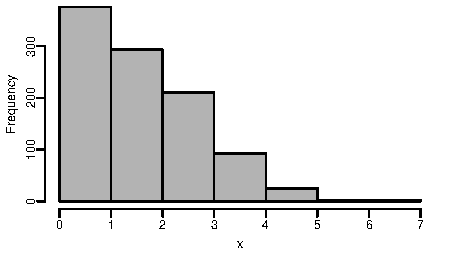
\includegraphics[width=\maxwidth]{figure/binom_freq-1} 

\end{knitrout}

\end{frame} 
%===============================================================================%

%===============================================================================
\begin{frame}[fragile]{Distribuição Binomial}

\small{Podemos também simular diferentes réplicas, e observar a frequência dos resultados:}


\begin{knitrout}\tiny
\definecolor{shadecolor}{rgb}{0.969, 0.969, 0.969}\color{fgcolor}\begin{kframe}
\begin{alltt}
\hlkwd{c}\hlstd{(p2,p3,p4); p2} \hlopt{+} \hlstd{p3} \hlopt{+} \hlstd{p4}
\end{alltt}
\begin{verbatim}
## [1] 0.30198989 0.20132659 0.08808038
## [1] 0.5913969
\end{verbatim}
\begin{alltt}
\hlkwd{hist}\hlstd{(x,}\hlkwc{breaks}\hlstd{=}\hlnum{7}\hlstd{,}\hlkwc{main}\hlstd{=}\hlnum{NA}\hlstd{,}\hlkwc{col}\hlstd{=}\hlstr{"gray70"}\hlstd{,}\hlkwc{freq}\hlstd{=F)}
\end{alltt}
\end{kframe}
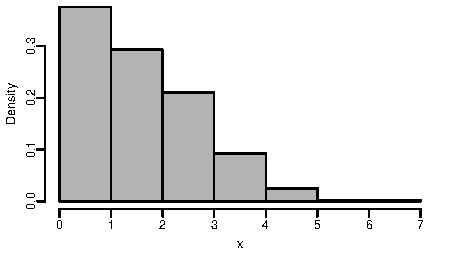
\includegraphics[width=\maxwidth]{figure/binom_freq2-1} 

\end{knitrout}

\end{frame} 
%===============================================================================%

%===============================================================================
\begin{frame}{Por que usar distribuições?}

\begin{itemize}
  \item Qual a vantagem de conhecermos uma distribuição de probabilidade?
  
\vfill

  \item Você espera que a maioria dos dados na natureza siga uma distribuição específica?
  
\vfill


\end{itemize}

\end{frame} 
%===============================================================================%


%===============================================================================
\begin{frame}{Por que usar distribuições?}

As distribuições possuem \textbf{propriedades conhecidas}. Para a Distribuição Binomial:

\vfill

\begin{small}

\textbf{Esperança (Primeiro Momento)}:
O valor "esperado" de uma V.A.
  \begin{equation*}
  E[X] = \sum_{i=1}^n{x_ip_i}
  \end{equation*}


\pause

\textbf{Variância (Segundo Momento)}:
A dispersão de uma V.A.
  \begin{equation*}
  Var[X] = \sum_{i=1}^n{p_i}(x_i - E[X])^2
  \end{equation*}


\end{small}

\end{frame} 
%===============================================================================%


%===============================================================================
\begin{frame}{Distribuição Binomial}

\textbf{Distribuição Binomial: $X \sim B(n,p)$}

Parâmetros: $n$ ($n \in \mathbb{N}$); $p$ ($0 < p < 1, p \in \mathbb{R}$)

Suporte: $x = k, k \in \left\{0,\ldots,n\right\}$

p.m.f:

\begin{equation*}
    f(x) = \binom{n}{k}p^k(1-p)^{n-k}
  \end{equation*}

$E[X] = np$

$Var[X] = np(1 - p)$

\end{frame} 
%===============================================================================%


%===============================================================================
\begin{frame}{Distribuição Binomial}



\textbf{Exemplo:} Se a probabilidade de captura é 0.2, qual o número médio de capturas eu espero obter após 10 visitas?

\begin{center}
$E[x] = np = 10 \times 0.2 = 2$ capturas
\end{center}

\textbf{Exemplo:} Como varia o número de capturas após 10 visitas?

\begin{center}
$Var[X] = np(1 - p) = 10 \times 0.2 \times (1 - 0.2) = 10 \times 0.2 \times 0.8 = 1.6$
\end{center}

\end{frame} 
%===============================================================================%

%===============================================================================
\begin{frame}[fragile]{Distribuição Binomial}

\begin{columns}[c]

\column{.3\textwidth}

$E[X] = 2$

\vfill

$Var[X] = 1.6$



\column{.7\textwidth}
\begin{knitrout}\tiny
\definecolor{shadecolor}{rgb}{0.969, 0.969, 0.969}\color{fgcolor}
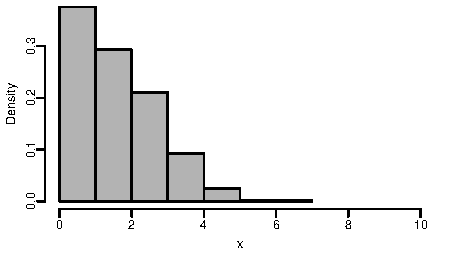
\includegraphics[width=\maxwidth]{figure/binom_plot-1} 

\end{knitrout}

\end{columns}



\end{frame} 
%===============================================================================%

%===============================================================================
\begin{frame}{Distribuição Binomial}

\begin{columns}[c]

\column{.3\textwidth}

$n = 10, p= 0.9$

\vfill

$E[X] = 9$

\vfill

$Var[X] = 0.9$

\column{.7\textwidth}

\begin{knitrout}\tiny
\definecolor{shadecolor}{rgb}{0.969, 0.969, 0.969}\color{fgcolor}
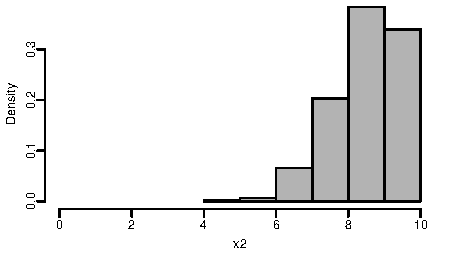
\includegraphics[width=\maxwidth]{figure/binom_plot2-1} 

\end{knitrout}

\end{columns}



\end{frame} 
%===============================================================================%

% %===============================================================================
% \begin{frame}[fragile]{Distribuições - por quê?}
% \begin{columns}[B]
% 
% \column{0.5\linewidth}
% 
% \begin{itemize}
%   \item A estatística foi desenvolvida antes dos computadores
% \vspace{0.25in}
%   \item Simulações eram extremamente trabalhosas
% \vspace{0.25in}
%   \item Assumir uma distribuição de probabilidade tornava os problemas tratáveis
% \end{itemize}
%   
% \column{0.5\linewidth}
% 
% <<binsim, fig.width=5,fig.height=4.3,out.width='0.7\\linewidth',size='tiny',echo=-1>>=
% par(mgp=c(1.8,0.5,0), mar=c(3,3,0,1),cex=1)
% n = 10; p = 0.2
% 
% E_x <- n*p; E_x
% 
% system.time(
%   sim <- rbinom(10000000,size=10,prob=0.2)
%   )
% 
% mean(sim)
% 
% hist(sim,breaks=c(0:10),xlim=c(0,10),main=NA)
% abline(v=mean(sim),col='red',lwd=2)
% @
% 
% 
% 
% \end{columns}
% 
% \end{frame} 
% %===============================================================================%

%===============================================================================
\begin{frame}{Distribuições Discretas}

\begin{small}

\begin{itemize}
  \item \textbf{Bernoulli} (Binomial com n=1): Sucesso em um evento.
    \vfill
  \item \textbf{Binomial} ($X \sim B(n,p$)): Sucesso em eventos sucessivos.
    \vfill
  \item \textbf{Multinomial} ($X \sim M(n,p_1,\dots,p_k)$): Generalização da binomial para mais de dois resultados possíveis.
    \vfill
  \item \textbf{Poisson} ($X \sim Pois(\lambda)$): Sucesso em um número desconhecido de eventos.
    \vfill
  \item \textbf{Binomial Negativa }($X \sim NB(r,p)$): Número de falhas acumuladas até que um certo número de sucessos ocorra.
    \vfill
  \item \textbf{Geométrica} ($X \sim Geom(p)$): Número de realizações até ocorrer uma falha.
    \vfill
  \item \textbf{Beta-binomial }($X \sim BetaBin(p,\theta)$): Binomial negativa com probabilidade de sucesso variável.
\end{itemize}

\end{small}

\end{frame} 
%===============================================================================%


%===============================================================================
\begin{frame}{Distribuição de Poisson}

\small{\textbf{Poisson}: A Binomial modela o número de sucessos esperados com um numero fixo de realizações. A distribuição Poisson modela a ocorrência de sucessos em situações onde o número de realizações é infinito. O exemplo mais comum são dados de contagem de indivíduos em parcelas, ou ao longo de um intervalo de tempo}. 

\vfill

\textbf{Distribuição Poisson:} $X \sim Pois(\lambda)$ 
  
Parâmetros: $\lambda$ ($\lambda > 0$)

Suporte: $x = k, k \in \left\{0,\ldots,n\right\}$

p.m.f:
  \begin{equation*}
    f(x) = \frac{lambda^k}{k!} e^{-\lambda}
  \end{equation*}

$E[X] = \lambda$

$Var[X] = \lambda$

\end{frame} 
%===============================================================================%

%===============================================================================
\begin{frame}[fragile]


Ex.: Se em média eu observo 50 indivíduos por parcela, qual a probabilidade de eu observar uma parcela com 100 indivíduos?

\begin{equation*}
  f(x) = \frac{lambda^k}{k!} e^{-\lambda}
\end{equation*}

\begin{equation*}
  P(x=100) = \frac{50^{100}}{100!} \times e^{-50}
\end{equation*}

\begin{equation*}
  P(x=100) = 845272575844 \times  1.92875 \times 10^{-22}
\end{equation*}

\begin{equation*}
  P(x=100) = 1.630319 \times 10^{-10}
\end{equation*}

\begin{knitrout}\tiny
\definecolor{shadecolor}{rgb}{0.969, 0.969, 0.969}\color{fgcolor}\begin{kframe}
\begin{alltt}
\hlkwd{dpois}\hlstd{(}\hlnum{100}\hlstd{,}\hlnum{50}\hlstd{)}
\end{alltt}
\begin{verbatim}
## [1] 1.630319e-10
\end{verbatim}
\end{kframe}
\end{knitrout}



\end{frame} 
%===============================================================================%


%===============================================================================
\begin{frame}{Distribuições Contínuas}

\begin{itemize}
  \item Até agora falamos de V.A. discretas
  \item Mas e se os dados que queremos modelar são contínuos?
  \item \textbf{Exemplo:} Qual a probabilidade da temperatura máxima de hoje ser 32$^\circ$C?
\end{itemize}

\end{frame} 
%===============================================================================%

%===============================================================================
\begin{frame}{Distribuições Contínuas}

\begin{itemize}
  \item Uma V.A. contínua pode assumir infinitos valores
  
  \vfill
  
  \item Se assumimos que: $P \approx F = \frac{n_i}{N}$
  
  \vfill
  
  \item Qual dos dois resultados tem probabilidade maior?
  
  \end{itemize}

\centering
  P(temperatura máxima de hoje) =  32$^\circ$C?
  
  ou
  
  P(temperatura máxima de hoje) = 32.354321$^\circ$C?
  
\end{frame} 
%===============================================================================%


%===============================================================================
\begin{frame}{Distribuições Contínuas}

Qual dos dois resultados tem probabilidade maior?
  \vfill
\centering

P(temperatura máxima de hoje) =  32$^\circ$C?
  
ou
  
P(temperatura máxima de hoje) = 32.354321$^\circ$C?

\vfill

Os dois tem a mesma probabilidade, que é \textbf{zero}.


$P(n_i) \approx F = \frac{n_i}{N} = \frac{1}{\inf} = 0

  
$ \lim_{N \to \inf} P(x) = 0$ 

\end{frame} 
%===============================================================================%



%===============================================================================
\begin{frame}{Distribuições Contínuas}


Para V.A. contínuas, ao invés de massas de probabilidade, falamos de \textbf{densidades de probabilidade}, dentro de um intervalo de valores.

\vfill

\item As distribuições de probabilidade contínuas tem, desta maneira, \textbf{funções de densidade de probabilidade (f.d.p ou \emph{p.d.f})}

\vfill

Qual a probabilidade da temperatura máxima de hoje estar entre 32 e 33$^\circ$C?

Qual a probabilidade da temperatura máxima de hoje ser maior que 32$^\circ$C?
    
\end{frame} 
%===============================================================================%

%===============================================================================
\begin{frame}{Distribuições Contínuas}

Qual a distribuição contínua mais utilizada? \pause

\vfill

\textbf{Distribuição Normal (Gaussiana): $X \sim N(\mu,\sigma)$}

\begin{footnotesize}

Parâmetros: $\mu$ ($\mu \in \mathbb{R})$); $\sigma$ ($\sigma > 0$)

Suporte: $X \in \mathbb{R}$

p.d.f:

\begin{equation*}
P(x) = \frac{1}{{\sigma \sqrt {2\pi } }}e^{{{ - \left( {x - \mu } \right)^2 } \mathord{\left/ {\vphantom {{ - \left( {x - \mu } \right)^2 } {2\sigma ^2 }}} \right. \kern-\nulldelimiterspace} {2\sigma ^2 }}}
\end{equation*}

$E(X) = \mu$

$Var(X) = \sigma^2$ (Muitas vezes usamos o desvio padrão: $\sqrt{\sigma^2} = \sigma$)



\alert{\textbf{Exemplo:}} Qual a probabilidade de observamos uma temperatura entre 30$^\circ$C e 35$^\circ$C, se a média histórica é $\mu = 30$, e o desvio padrão é $\sigma = 5$?

\end{footnotesize}
    
\end{frame} 
%===============================================================================%

%===============================================================================
\begin{frame}[fragile]{Distribuição Normal - Exemplo}


\begin{knitrout}
\definecolor{shadecolor}{rgb}{0.969, 0.969, 0.969}\color{fgcolor}
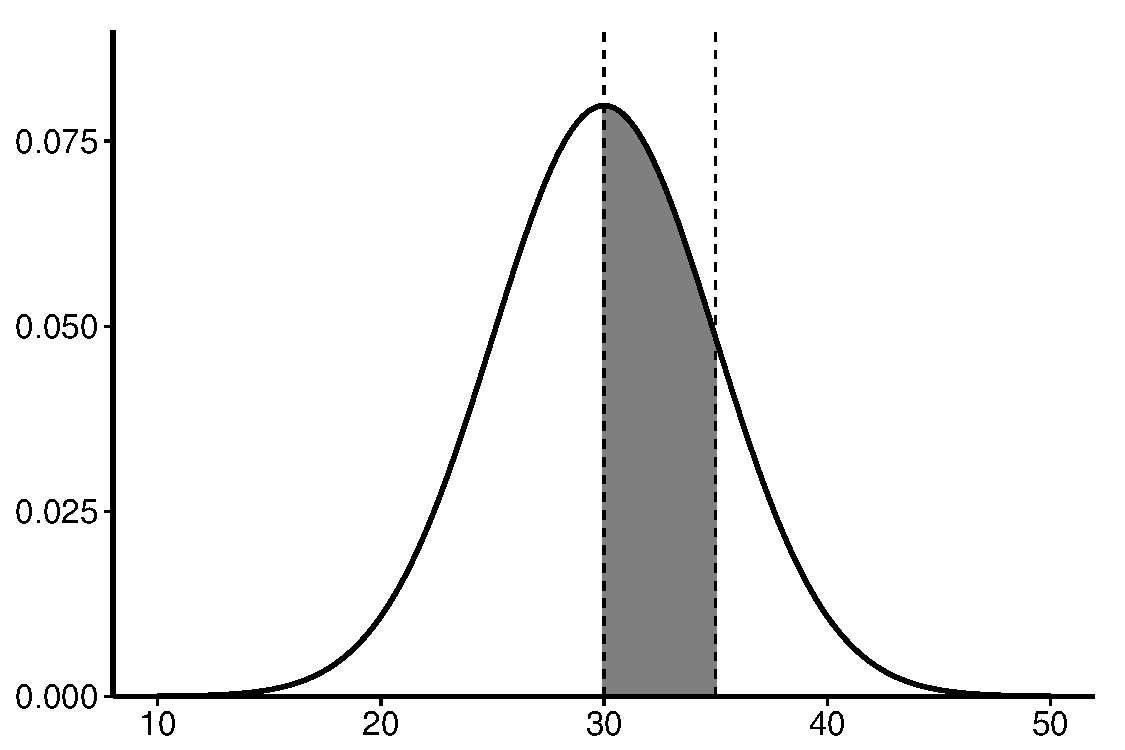
\includegraphics[width=\maxwidth,height=0.7\textheight]{figure/normex-1} 

\end{knitrout}

\end{frame} 
%===============================================================================%


%===============================================================================
\begin{frame}[fragile]{Distribuição Normal - Exemplo}


\begin{knitrout}\tiny
\definecolor{shadecolor}{rgb}{0.969, 0.969, 0.969}\color{fgcolor}\begin{kframe}
\begin{alltt}
\hlcom{# No R}
\hlstd{media} \hlkwb{<-} \hlnum{30}
\hlstd{desvio} \hlkwb{<-} \hlnum{5}
\hlstd{tmin} \hlkwb{<-} \hlnum{30}
\hlstd{tmax} \hlkwb{<-} \hlnum{35}

\hlcom{# A maneira mais fácil de calcular uma probabilidade é de maneira cumulativa: P(x <= 30)}
\hlcom{#O comando "pnorm" faz isso:}

\hlstd{p.tmin} \hlkwb{<-} \hlkwd{pnorm}\hlstd{(tmin,}\hlkwc{mean}\hlstd{=media,}\hlkwc{sd}\hlstd{=desvio)}

\hlstd{p.tmin}
\end{alltt}
\begin{verbatim}
## [1] 0.5
\end{verbatim}
\end{kframe}
\end{knitrout}

\end{frame} 
%===============================================================================%


%===============================================================================
\begin{frame}[fragile]{Distribuição Normal - Exemplo}

\begin{knitrout}
\definecolor{shadecolor}{rgb}{0.969, 0.969, 0.969}\color{fgcolor}
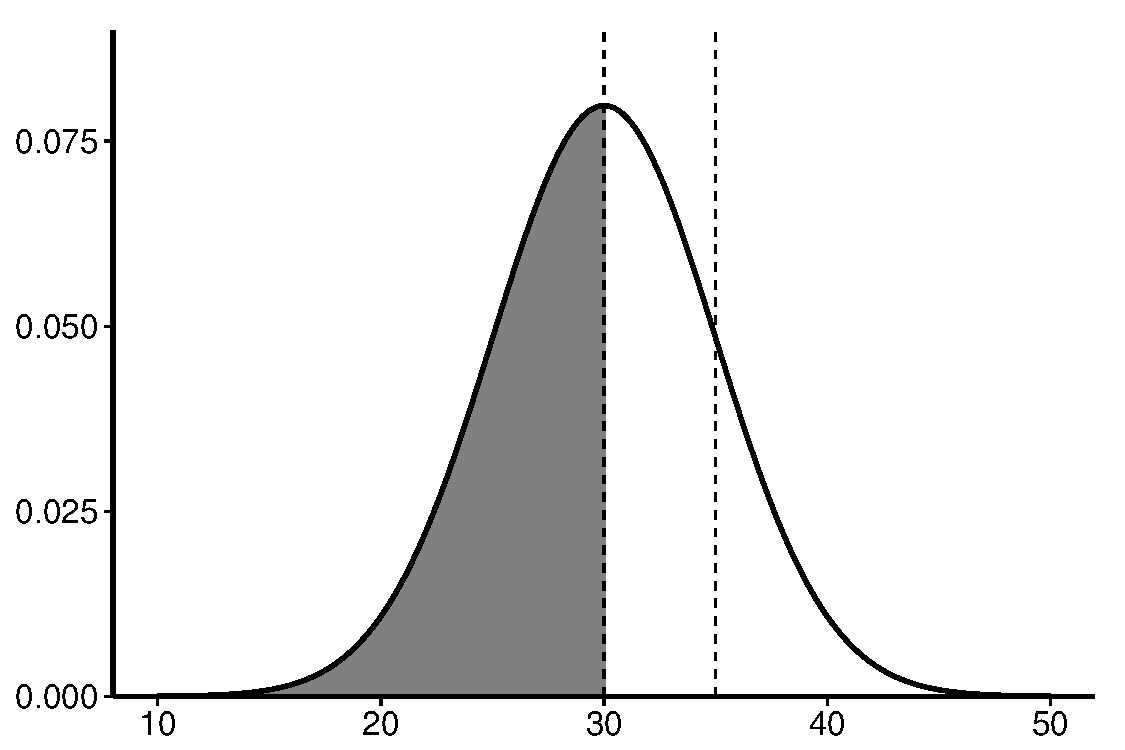
\includegraphics[width=\maxwidth,height=0.7\textheight]{figure/cumnormplot1-1} 

\end{knitrout}

\end{frame} 
%===============================================================================%

%===============================================================================
\begin{frame}[fragile]{Distribuição Normal - Exemplo}


\begin{knitrout}\tiny
\definecolor{shadecolor}{rgb}{0.969, 0.969, 0.969}\color{fgcolor}\begin{kframe}
\begin{alltt}
\hlcom{# No R}
\hlstd{media} \hlkwb{<-} \hlnum{30}
\hlstd{desvio} \hlkwb{<-} \hlnum{5}
\hlstd{tmin} \hlkwb{<-} \hlnum{30}
\hlstd{tmax} \hlkwb{<-} \hlnum{35}

\hlcom{# calculamos também a probabilidade cumulativa de x <= 35}

\hlstd{p.tmax} \hlkwb{<-} \hlkwd{pnorm}\hlstd{(tmax,}\hlkwc{mean}\hlstd{=media,}\hlkwc{sd}\hlstd{=desvio)}

\hlstd{p.tmax}
\end{alltt}
\begin{verbatim}
## [1] 0.8413447
\end{verbatim}
\end{kframe}
\end{knitrout}

\end{frame} 
%===============================================================================%


%===============================================================================
\begin{frame}[fragile]{Distribuição Normal - Exemplo}

\begin{knitrout}
\definecolor{shadecolor}{rgb}{0.969, 0.969, 0.969}\color{fgcolor}
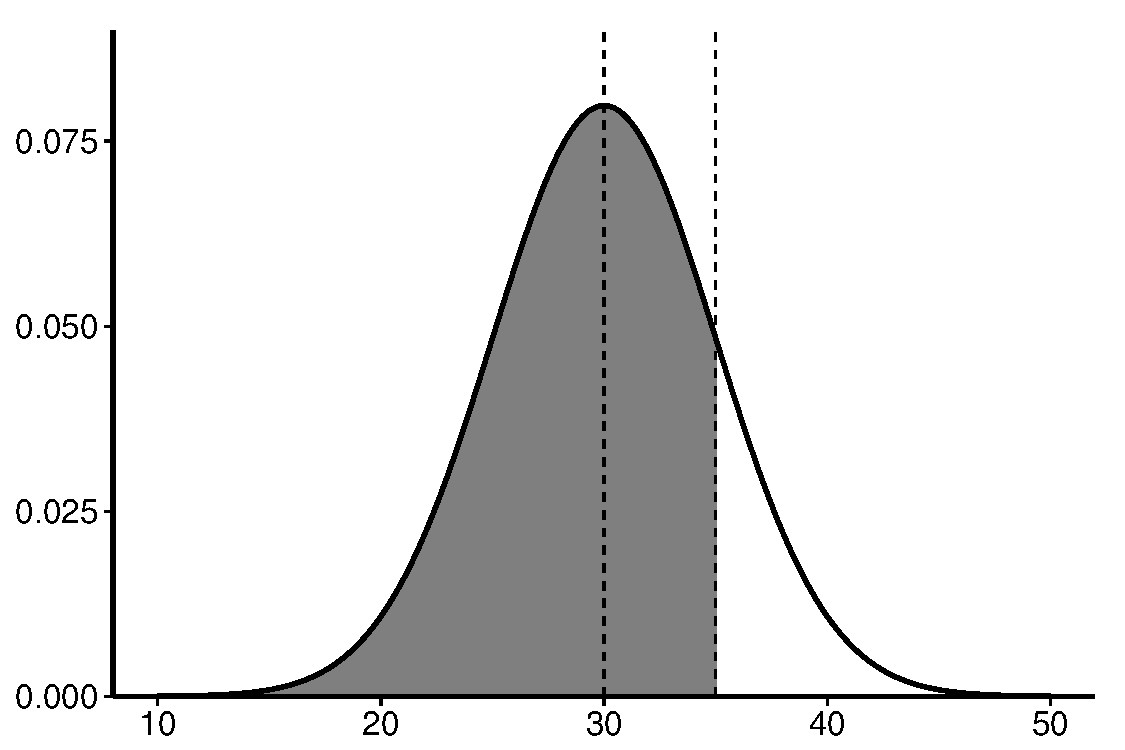
\includegraphics[width=\maxwidth,height=0.7\textheight]{figure/cumnormplot2-1} 

\end{knitrout}

\end{frame} 
%===============================================================================%

%===============================================================================
\begin{frame}[fragile]{Distribuição Normal - Exemplo}


\begin{knitrout}\tiny
\definecolor{shadecolor}{rgb}{0.969, 0.969, 0.969}\color{fgcolor}\begin{kframe}
\begin{alltt}
\hlcom{# Sabendo as duas probabilidades cumulativas, é só subtrair}

\hlstd{p.tmax} \hlopt{-} \hlstd{p.tmin}
\end{alltt}
\begin{verbatim}
## [1] 0.3413447
\end{verbatim}
\end{kframe}
\end{knitrout}

\end{frame} 
%===============================================================================%


%===============================================================================
\begin{frame}[fragile]{Distribuição Normal - Exemplo}

\begin{knitrout}
\definecolor{shadecolor}{rgb}{0.969, 0.969, 0.969}\color{fgcolor}
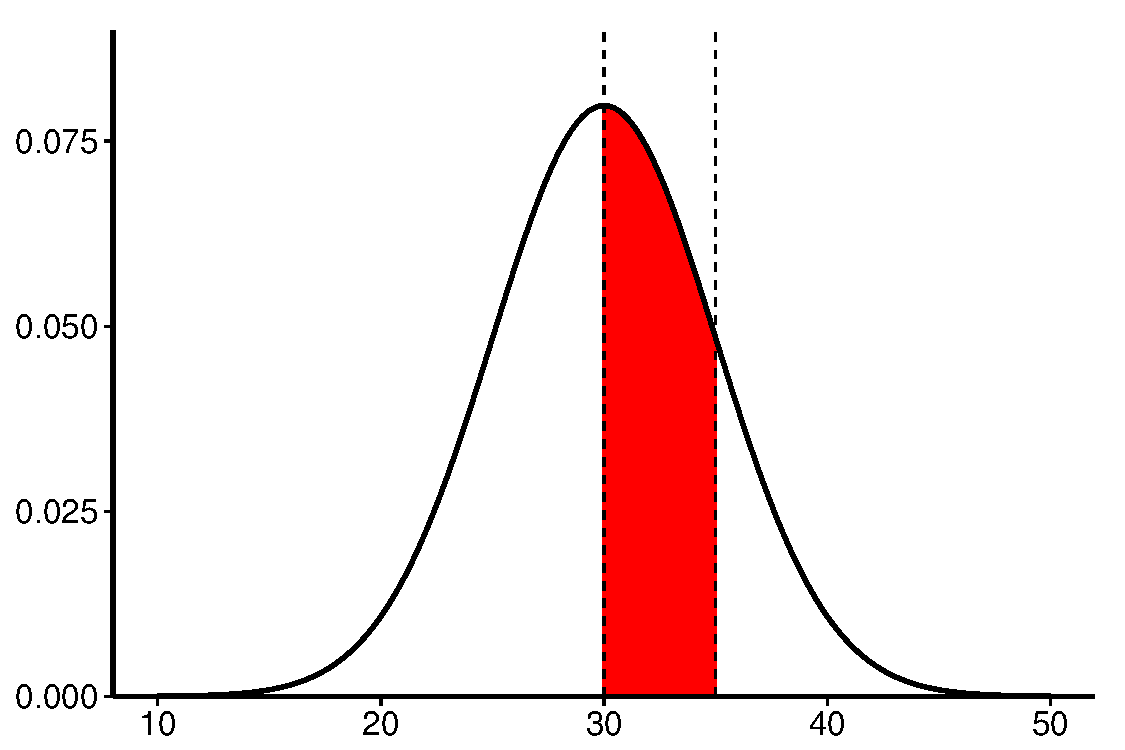
\includegraphics[width=\maxwidth,height=0.7\textheight]{figure/cumnormplot3-1} 

\end{knitrout}

\end{frame} 
%===============================================================================%


%===============================================================================
\begin{frame}{Distribuições Contínuas}

\begin{small}
\begin{itemize}
  \item \textbf{Normal}: $X \sim N(\mu,\sigma)$
  \vfill
  \item \textbf{Gamma}: $X \sim Gamma(s,a$)
  \vfill
  \item \textbf{Exponencial}: $X \sim Exp(\lambda)$
  \vfill
  \item \textbf{Beta}: $X \sim Beta(a,b)$
  \vfill
  \item \textbf{Lognormal}: $X \sim logN(\mu,\sigma)$
  \vfill
  \item \textbf{Qui-quadrado}: $X \sim \chi^2(df)$
\end{itemize}
\end{small}

\end{frame} 
%===============================================================================%

\section{Testes de Hipóteses}


%===============================================================================
\begin{frame}{Testes de Hipóteses Paramétricos}

O mecanismo dos testes de hipóteses \textbf{paramétricos} seguem sempre a mesma lógica:
\vfill
  \begin{small}
  \begin{enumerate}
    \item Formule uma hipótese quantitativa \pause
    \item Defina uma estatística de interesse que descreva essa quantidade \pause
    \item Assuma uma distribuição para esta estatística de interesse, caso a hipótese seja verdadeira
    \item Especifique os parâmetros dessa distribuição \pause
    \item Calcule a probabilidade de se obter a estatística de interesse observada, \textbf{ou uma mais extrema}, a partir da sua amostra, se a sua hipótese for verdadeira. \pause
    \item Avalie a "força da evidência" em relação sua hipótese, com base na probabilidade observada para a amostra. \pause
  \end{enumerate}
  \end{small}
  
\end{frame} 
%===============================================================================%

%===============================================================================
\begin{frame}{Exemplo: Teste dos Sinais}

\textbf{Pergunta:} Estou comparando duas amostras pareadas ($X,Y$), com $N$ observações, e quero saber se existe diferença entre elas.
\medskip

\textbf{Hipótese:} Se não há diferença, $P(x_i > y_i) = P(y_i > x_i) = 0.5$. Podemos pensar em $x_i > y_i$ como um sucesso, e $y_i > x_i$ como um fracasso
\medskip

\textbf{Estatística de interesse - W}: quantas vezes observamos $x_i > y_i$?
\medskip

\only<1-1>{\textbf{Distribuição de W?}}
\only<2-2>{\textbf{Distribuição de W:} $W ~ Bin(n=N,p=0.5)$}
\medskip

\only<2-2>{Qual a probabilidade de obtermos o valor observado de W ou maior, na nossa amostra, se $W ~ Bin(n=N,p=0.5)$?}


\end{frame} 
%===============================================================================%


%===============================================================================
\begin{frame}[fragile]{Exemplo:Teste dos Sinais}


\begin{knitrout}\tiny
\definecolor{shadecolor}{rgb}{0.969, 0.969, 0.969}\color{fgcolor}\begin{kframe}
\begin{alltt}
\hlstd{x} \hlkwb{<-} \hlkwd{c}\hlstd{(}\hlnum{0}\hlstd{,}\hlnum{3}\hlstd{,}\hlnum{6}\hlstd{,}\hlnum{5}\hlstd{,}\hlnum{3}\hlstd{,}\hlnum{7}\hlstd{,}\hlnum{8}\hlstd{,}\hlnum{9}\hlstd{,}\hlnum{2}\hlstd{,}\hlnum{4}\hlstd{,}\hlnum{6}\hlstd{,}\hlnum{7}\hlstd{)}
\hlstd{y} \hlkwb{<-} \hlkwd{c}\hlstd{(}\hlnum{3}\hlstd{,}\hlnum{4}\hlstd{,}\hlnum{5}\hlstd{,}\hlnum{6}\hlstd{,}\hlnum{9}\hlstd{,}\hlnum{7}\hlstd{,}\hlnum{1}\hlstd{,}\hlnum{2}\hlstd{,}\hlnum{3}\hlstd{,}\hlnum{4}\hlstd{,}\hlnum{5}\hlstd{,}\hlnum{6}\hlstd{)}

\hlstd{n}\hlkwb{=}\hlkwd{length}\hlstd{(x); n}
\end{alltt}
\begin{verbatim}
## [1] 12
\end{verbatim}
\begin{alltt}
\hlstd{d} \hlkwb{<-} \hlstd{x}\hlopt{-}\hlstd{y; d}
\end{alltt}
\begin{verbatim}
##  [1] -3 -1  1 -1 -6  0  7  7 -1  0  1  1
\end{verbatim}
\begin{alltt}
\hlstd{w} \hlkwb{<-} \hlkwd{sum}\hlstd{(x}\hlopt{-}\hlstd{y} \hlopt{>} \hlnum{0}\hlstd{); w}
\end{alltt}
\begin{verbatim}
## [1] 5
\end{verbatim}
\begin{alltt}
\hlkwd{dbinom}\hlstd{(w,}\hlkwc{size}\hlstd{=}\hlnum{12}\hlstd{,}\hlkwc{prob}\hlstd{=}\hlnum{0.5}\hlstd{)}
\end{alltt}
\begin{verbatim}
## [1] 0.1933594
\end{verbatim}
\end{kframe}
\end{knitrout}

\end{frame} 
%===============================================================================%

  
%===============================================================================
\begin{frame}[fragile]{Exemplo:Teste dos Sinais}

\begin{knitrout}\tiny
\definecolor{shadecolor}{rgb}{0.969, 0.969, 0.969}\color{fgcolor}\begin{kframe}
\begin{alltt}
\hlcom{# Mas eu quero saber P(w >= 5)}

\hlstd{probs} \hlkwb{<-}\hlkwd{vector}\hlstd{(}\hlnum{8}\hlstd{,}\hlkwc{mode}\hlstd{=}\hlstr{'numeric'}\hlstd{)}

\hlkwa{for}\hlstd{(i} \hlkwa{in} \hlkwd{c}\hlstd{(}\hlnum{5}\hlopt{:}\hlnum{12}\hlstd{))\{}
  \hlstd{w}\hlkwb{=}\hlstd{i}
  \hlstd{probs[i]} \hlkwb{<-} \hlkwd{dbinom}\hlstd{(w,}\hlkwc{size}\hlstd{=}\hlnum{12}\hlstd{,}\hlkwc{prob}\hlstd{=}\hlnum{0.5}\hlstd{)}
\hlstd{\}}

\hlstd{probs}
\end{alltt}
\begin{verbatim}
##  [1] 0.0000000000 0.0000000000 0.0000000000 0.0000000000 0.1933593750
##  [6] 0.2255859375 0.1933593750 0.1208496094 0.0537109375 0.0161132813
## [11] 0.0029296875 0.0002441406
\end{verbatim}
\begin{alltt}
\hlkwd{sum}\hlstd{(probs)}
\end{alltt}
\begin{verbatim}
## [1] 0.8061523
\end{verbatim}
\end{kframe}
\end{knitrout}

\end{frame} 
%===============================================================================%

%===============================================================================
\begin{frame}[fragile]{Exemplo:Teste dos Sinais}

\begin{knitrout}\tiny
\definecolor{shadecolor}{rgb}{0.969, 0.969, 0.969}\color{fgcolor}\begin{kframe}
\begin{alltt}
\hlkwd{binom.test}\hlstd{(}\hlnum{5}\hlstd{,}\hlnum{12}\hlstd{,}\hlkwc{p}\hlstd{=}\hlnum{0.5}\hlstd{,}\hlkwc{alternative}\hlstd{=}\hlstr{"greater"}\hlstd{)}
\end{alltt}
\begin{verbatim}
## 
## 	Exact binomial test
## 
## data:  5 and 12
## number of successes = 5, number of trials = 12, p-value = 0.8062
## alternative hypothesis: true probability of success is greater than 0.5
## 95 percent confidence interval:
##  0.1810248 1.0000000
## sample estimates:
## probability of success 
##              0.4166667
\end{verbatim}
\end{kframe}
\end{knitrout}

\end{frame} 
%===============================================================================%


%===============================================================================
\begin{frame}{Exemplo: Teste $\chi^2$}


\textbf{Teste  $\chi^2$ (chi-quadrado, chi pronuncia-se "qui")}

\begin{footnotesize}

\textbf{Pergunta:} Contei os indivíduos em 3 habitats: $N_F=86$,$N_P=3$,$N_A=11$. Cada habitat estava representado na seguinte proporção: Floresta(75\%), Pastagem (10\%), Agricultura(15\%) . Será que existe uma preferência dos indivíduos por um determinado habitat?


\textbf{Hipótese:} Se não há preferência, a quantidade esperada de indivíduos em cada habitat só é afetada  pela proporção de cada um. Se a quantidade observada for diferente da esperada, há indício de preferência.


\textbf{Estatística:} $X^2 = \sum{\frac{(O-E)^2}{E}}$

\textbf{Distribuição de $X^2$:} $X^2 \sim \chi^2(k)$ ($k$ =  graus de liberdade = $N -1$)


Qual a probabilidade de obtermos o valor observado de $X^2$ ou mais extremo, na nossa amostra?


\end{footnotesize}

\end{frame} 
%===============================================================================%


%===============================================================================
\begin{frame}[fragile]

\begin{knitrout}\tiny
\definecolor{shadecolor}{rgb}{0.969, 0.969, 0.969}\color{fgcolor}\begin{kframe}
\begin{alltt}
\hlstd{obs} \hlkwb{<-} \hlkwd{c}\hlstd{(}\hlnum{86}\hlstd{,}\hlnum{3}\hlstd{,}\hlnum{11}\hlstd{)}
\hlstd{habs} \hlkwb{<-} \hlkwd{c}\hlstd{(}\hlnum{0.75}\hlstd{,}\hlnum{0.1}\hlstd{,}\hlnum{0.15}\hlstd{)}
\hlstd{esp} \hlkwb{<-} \hlkwd{rep}\hlstd{(}\hlkwd{sum}\hlstd{(obs),}\hlnum{3}\hlstd{)} \hlopt{*} \hlstd{habs}

\hlstd{x2} \hlkwb{<-} \hlkwd{sum}\hlstd{((obs}\hlopt{-}\hlstd{esp)}\hlopt{^}\hlnum{2}\hlopt{/}\hlstd{(esp))}
\hlstd{x2}
\end{alltt}
\begin{verbatim}
## [1] 7.58
\end{verbatim}
\begin{alltt}
\hlkwd{dchisq}\hlstd{(x2,}\hlkwc{df}\hlstd{=}\hlnum{2}\hlstd{)}
\end{alltt}
\begin{verbatim}
## [1] 0.0112978
\end{verbatim}
\begin{alltt}
\hlcom{# A distribuição qui-quadrada é contínua, então não dá pra somar. Mas existe uma função cumulativa:}
\hlnum{1}\hlopt{-}\hlkwd{pchisq}\hlstd{(x2,}\hlkwc{df}\hlstd{=}\hlnum{2}\hlstd{)}
\end{alltt}
\begin{verbatim}
## [1] 0.0225956
\end{verbatim}
\begin{alltt}
\hlkwd{chisq.test}\hlstd{(obs,}\hlkwc{p}\hlstd{=habs)}
\end{alltt}
\begin{verbatim}
## 
## 	Chi-squared test for given probabilities
## 
## data:  obs
## X-squared = 7.58, df = 2, p-value = 0.0226
\end{verbatim}
\end{kframe}
\end{knitrout}

\end{frame} 
%===============================================================================%


%===============================================================================
\begin{frame}{Exemplo: Teste Z para a média}

\begin{block}{Pergunta}

Um reservatório com concentrações de clorofila maiores do que 3 mg.m$^{-3}$ pode ser considerado eutrófico. Eu coleto 20 amostras de água e determino uma concentração média de 2.55 mg.m$^{-3}$, com um desvio padrão de 0.9 mg.m$^{-3}$. Será que meu reservatório é eutrófico? 

\end{block}

\end{frame} 
%===============================================================================%

%===============================================================================
\begin{frame}{Exemplo: Teste Z para a média}

\textbf{H$_0$:} O reservatório está contaminado, então $\mu = 3$
\vfill
\textbf{H$_1$:} O reservatório não está contaminado, então $\mu < 3$
\vfill
$P(\bar{X} >= 2.55 | \mu = 3)$?
\vfill

\textbf{Estatística:} $Z$

\vfill

\begin{equation*}
    Z = \frac{\bar{X} - \mu}{E.P.} = \frac{\bar{X} - \mu}{\sigma / \sqrt{n}}
\end{equation*}

\vfill

\only<1-1>{\textbf{Distribuição de $Z$?}}
\only<2-2>{\textbf{Distribuição de $Z$:}  $Z \sim N (0,1)$}

\end{frame} 
%===============================================================================%

%===============================================================================
\begin{frame}{Erro Padrão vs. Desvio Padrão}

\begin{small}
  
  \item Uma confusão comum é confundir desvio padrão (\emph{standard deviation}) e erro padrão (\emph{standard error}). Qual a diferença? \pause
  \vfill
  \item O desvio padrão mede a dispersão dos dados observados.
  \vfill
  \item A partir desses dados, podemos calcular a média ($\bar{X}$), um estimador da média da população ($\mu$). Se tomarmos amostras diferentes, teremos $\bar{X}$ diferentes. Qual a distribuição de $\bar{X}$?
  \pause
  \item O erro padrão mede a dispersão esperada (desvio padrão) de $\bar{X}$, não dos dados originais

\end{small}

\vfill

\textbf{Erro Padrão da Média}:
\centering
$ E.P. = \frac{\sigma}{\sqrt{n}}$ 

\end{frame} 
%===============================================================================%


%===============================================================================
\begin{frame}[fragile]{Desvio padrão vs. erro padrão}


\begin{knitrout}\tiny
\definecolor{shadecolor}{rgb}{0.969, 0.969, 0.969}\color{fgcolor}\begin{kframe}
\begin{alltt}
\hlcom{# Tomamos uma amostra aleatória com X ~ N(30,5) e n=50}
\hlkwd{set.seed}\hlstd{(}\hlnum{20}\hlstd{)}
\hlstd{x} \hlkwb{<-} \hlkwd{rnorm}\hlstd{(}\hlnum{20}\hlstd{,}\hlnum{30}\hlstd{,}\hlnum{5}\hlstd{); x}
\end{alltt}
\begin{verbatim}
##  [1] 35.81343 27.07038 38.92733 23.33703 27.76717 32.84803 15.55141 25.65491
##  [9] 27.69149 27.22230 29.89932 29.24809 26.85937 36.61610 22.39325 27.81286
## [17] 34.85289 30.14111 29.57109 31.94607
\end{verbatim}
\begin{alltt}
\hlcom{# Calculamos a média e o desvio padrão}
\hlstd{x_barra} \hlkwb{<-} \hlkwd{mean}\hlstd{(x); x_barra}
\end{alltt}
\begin{verbatim}
## [1] 29.06118
\end{verbatim}
\begin{alltt}
\hlstd{s} \hlkwb{<-} \hlkwd{sd}\hlstd{(x); s}
\end{alltt}
\begin{verbatim}
## [1] 5.365711
\end{verbatim}
\end{kframe}
\end{knitrout}

\end{frame} 
%===============================================================================%

%===============================================================================
\begin{frame}[fragile]{Desvio padrão vs. erro padrão}

\begin{knitrout}
\definecolor{shadecolor}{rgb}{0.969, 0.969, 0.969}\color{fgcolor}
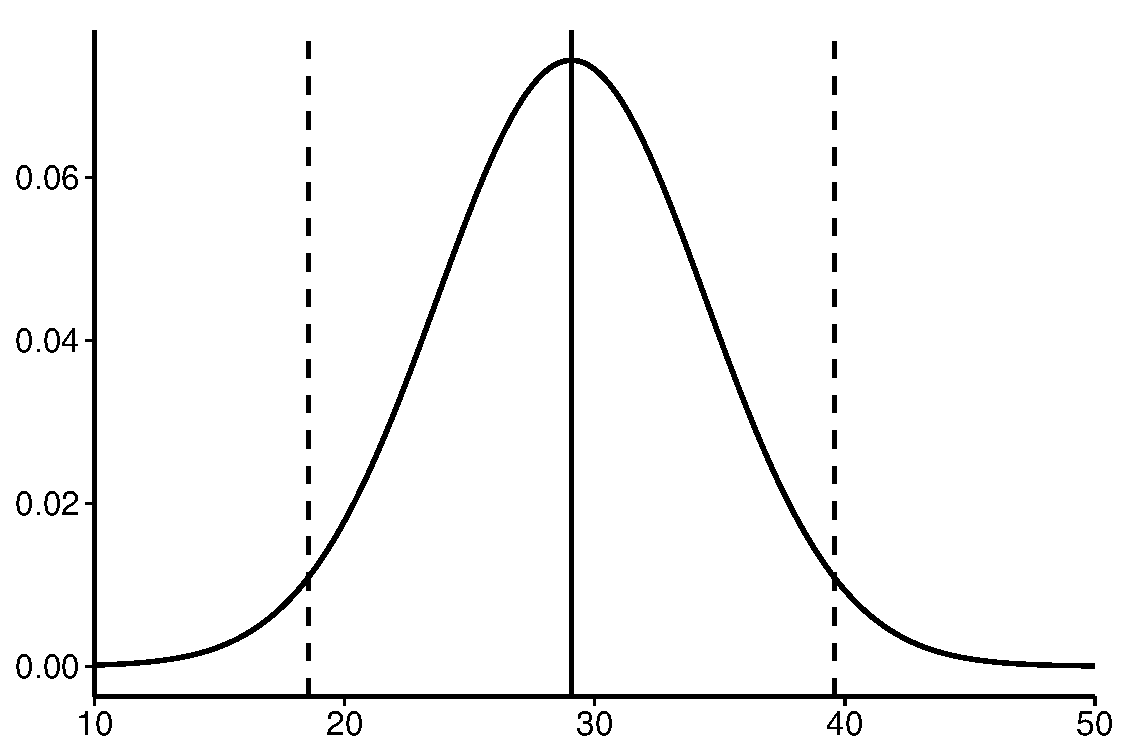
\includegraphics[width=\maxwidth,height=0.7\textheight]{figure/desv_err_plot1-1} 

\end{knitrout}

\end{frame} 
%===============================================================================%

%===============================================================================
\begin{frame}[fragile]{Desvio padrão vs. erro padrão}


\begin{knitrout}\tiny
\definecolor{shadecolor}{rgb}{0.969, 0.969, 0.969}\color{fgcolor}\begin{kframe}
\begin{alltt}
\hlcom{# Mas podemos repetir essa amostragem 10000 vezes, e ter 10000 médias diferentes}
\hlstd{medias} \hlkwb{<-} \hlkwd{vector}\hlstd{(}\hlnum{10000}\hlstd{,}\hlkwc{mode}\hlstd{=}\hlstr{'numeric'}\hlstd{)}

\hlkwa{for} \hlstd{(i} \hlkwa{in} \hlkwd{c}\hlstd{(}\hlnum{1}\hlopt{:}\hlnum{10000}\hlstd{))\{}
  \hlstd{x} \hlkwb{<-} \hlkwd{rnorm}\hlstd{(}\hlnum{20}\hlstd{,}\hlnum{30}\hlstd{,}\hlnum{5}\hlstd{)}
  \hlstd{medias[i]} \hlkwb{<-} \hlkwd{mean}\hlstd{(x)}
\hlstd{\}}

\hlkwd{mean}\hlstd{(medias)}
\end{alltt}
\begin{verbatim}
## [1] 29.99082
\end{verbatim}
\begin{alltt}
\hlkwd{sd}\hlstd{(medias)}
\end{alltt}
\begin{verbatim}
## [1] 1.103708
\end{verbatim}
\end{kframe}
\end{knitrout}

\end{frame} 
%===============================================================================%

%===============================================================================
\begin{frame}[fragile]{Desvio padrão vs. erro padrão}

\begin{knitrout}
\definecolor{shadecolor}{rgb}{0.969, 0.969, 0.969}\color{fgcolor}
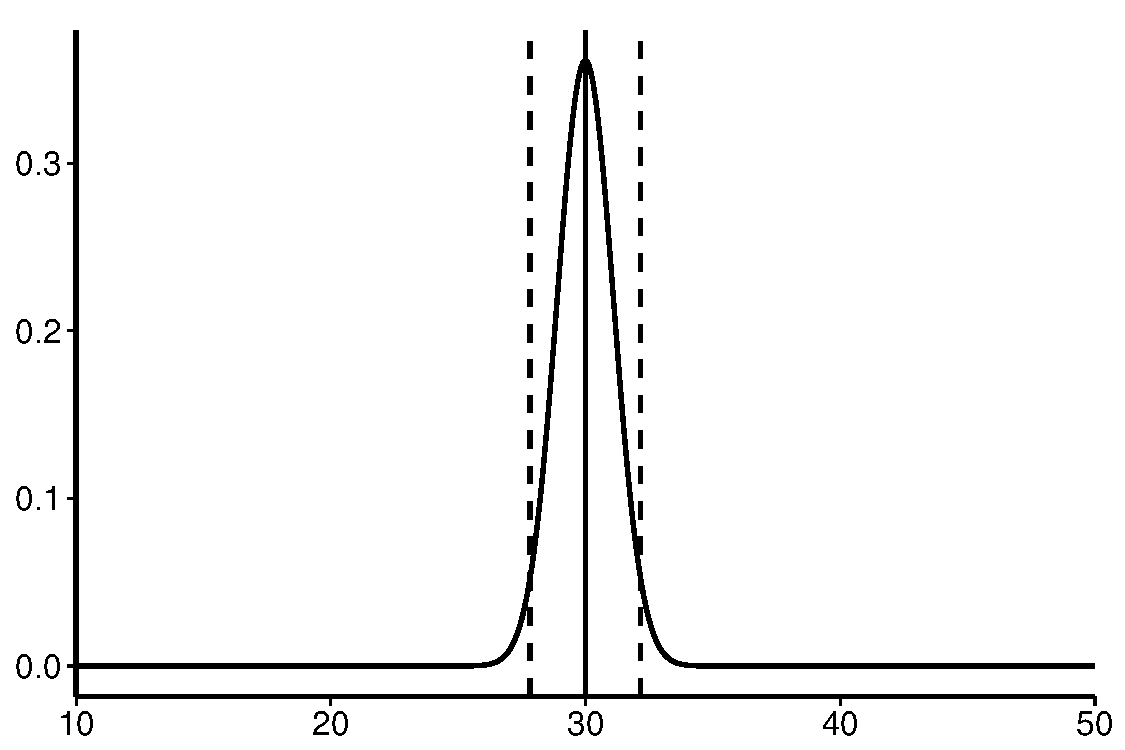
\includegraphics[width=\maxwidth,height=0.7\textheight]{figure/desv_err_plot2-1} 

\end{knitrout}

\end{frame} 
%===============================================================================%

%===============================================================================
\begin{frame}[fragile]{Desvio padrão vs. erro padrão}

\begin{knitrout}
\definecolor{shadecolor}{rgb}{0.969, 0.969, 0.969}\color{fgcolor}
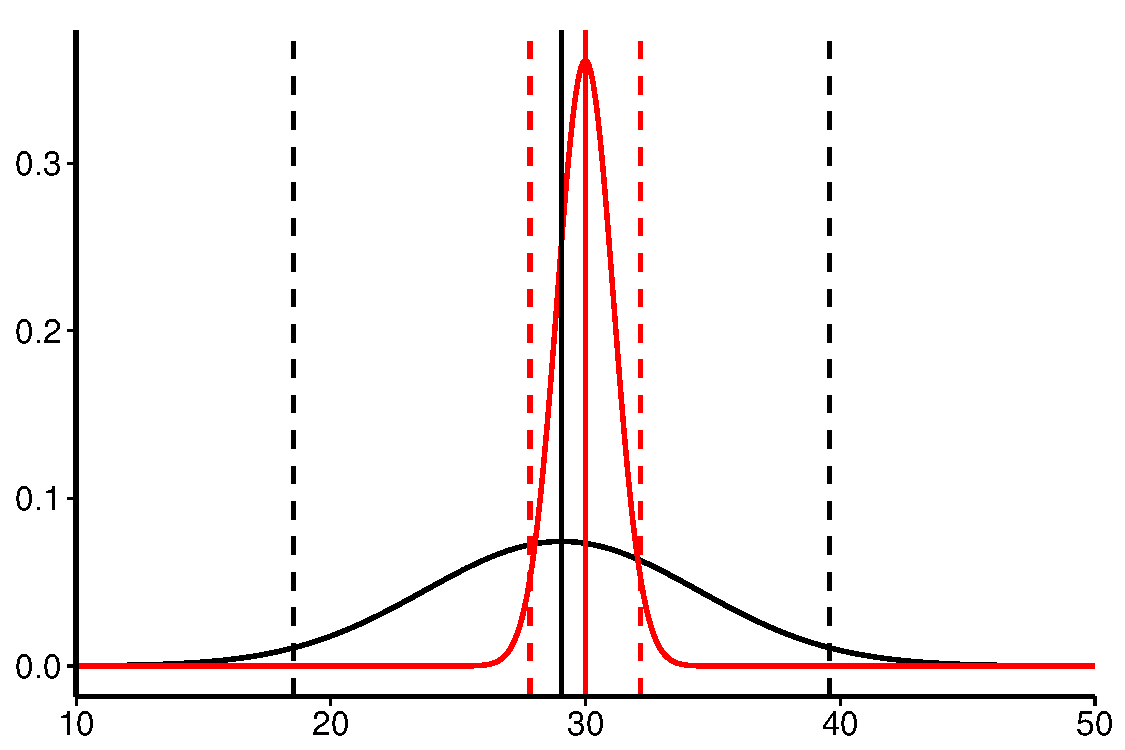
\includegraphics[width=\maxwidth,height=0.7\textheight]{figure/desv_err_plot3-1} 

\end{knitrout}

\end{frame} 
%===============================================================================%

%===============================================================================
\begin{frame}[fragile]{Desvio padrão vs. erro padrão}


\begin{knitrout}\scriptsize
\definecolor{shadecolor}{rgb}{0.969, 0.969, 0.969}\color{fgcolor}\begin{kframe}
\begin{alltt}
\hlcom{# De fato}

\hlkwd{sd}\hlstd{(medias)}
\end{alltt}
\begin{verbatim}
## [1] 1.103708
\end{verbatim}
\begin{alltt}
\hlnum{5}\hlopt{/}\hlkwd{sqrt}\hlstd{(}\hlnum{20}\hlstd{)}
\end{alltt}
\begin{verbatim}
## [1] 1.118034
\end{verbatim}
\end{kframe}
\end{knitrout}

\end{frame} 
%===============================================================================%


%===============================================================================
\begin{frame}{Exemplo: Teste Z para a média}

\textbf{H$_0$:} O reservatório está contaminado, então $\mu = 3$
\vfill
\textbf{H$_1$:} O reservatório não está contaminado, então $\mu < 3$
\vfill
$P(\bar{X} >= 2.55 | \mu = 3)$?
\vfill

\textbf{Estatística:} $Z$

\vfill

\begin{equation*}
    Z = \frac{\bar{X} - \mu}{E.P.} = \frac{\bar{X} - \mu}{\sigma / \sqrt{n}}
\end{equation*}

\vfill

\only<1-1>{\textbf{Distribuição de $Z$?}}
\only<2-2>{\textbf{Distribuição de $Z$:}  $Z \sim N (0,1)$}

\end{frame} 
%===============================================================================%

%===============================================================================
\begin{frame}[fragile]{Exemplo: Teste Z para a média}

\begin{knitrout}\tiny
\definecolor{shadecolor}{rgb}{0.969, 0.969, 0.969}\color{fgcolor}\begin{kframe}
\begin{alltt}
\hlstd{n} \hlkwb{=} \hlnum{20}
\hlstd{x} \hlkwb{<-}  \hlkwd{c}\hlstd{(}\hlnum{1.85}\hlstd{,} \hlnum{2.64}\hlstd{,} \hlnum{3.63}\hlstd{,} \hlnum{1.94}\hlstd{,} \hlnum{2.41}\hlstd{,} \hlnum{2.74}\hlstd{,} \hlnum{2.85}\hlstd{,} \hlnum{3.07}\hlstd{,} \hlnum{1.29}\hlstd{,}
        \hlnum{1.50}\hlstd{,} \hlnum{1.55}\hlstd{,} \hlnum{1.69}\hlstd{,} \hlnum{3.70}\hlstd{,} \hlnum{3.25}\hlstd{,} \hlnum{2.47}\hlstd{,} \hlnum{1.95}\hlstd{,} \hlnum{3.33}\hlstd{,} \hlnum{2.21}\hlstd{,} \hlnum{3.02}\hlstd{,} \hlnum{3.98}\hlstd{)}
\hlstd{x_barra} \hlkwb{<-} \hlkwd{mean}\hlstd{(x)}
\hlstd{x_barra}
\end{alltt}
\begin{verbatim}
## [1] 2.5535
\end{verbatim}
\begin{alltt}
\hlstd{s} \hlkwb{<-} \hlkwd{sd}\hlstd{(x)}
\hlstd{s}
\end{alltt}
\begin{verbatim}
## [1] 0.7964016
\end{verbatim}
\begin{alltt}
\hlstd{mu} \hlkwb{<-} \hlnum{3}

\hlstd{x_barra}\hlopt{-}\hlstd{mu}
\end{alltt}
\begin{verbatim}
## [1] -0.4465
\end{verbatim}
\begin{alltt}
\hlstd{(x_barra}\hlopt{-}\hlstd{mu)}\hlopt{/}\hlstd{(s}\hlopt{/}\hlkwd{sqrt}\hlstd{(n))}
\end{alltt}
\begin{verbatim}
## [1] -2.507289
\end{verbatim}
\end{kframe}
\end{knitrout}
\end{frame} 
%===============================================================================%

%===============================================================================
\begin{frame}[fragile]{Exemplo: Teste Z para a média}
\begin{knitrout}\tiny
\definecolor{shadecolor}{rgb}{0.969, 0.969, 0.969}\color{fgcolor}\begin{kframe}
\begin{alltt}
\hlstd{z} \hlkwb{<-} \hlstd{(x_barra}\hlopt{-}\hlstd{mu)}\hlopt{/}\hlstd{(s}\hlopt{/}\hlkwd{sqrt}\hlstd{(n))}

\hlkwd{pnorm}\hlstd{(z,}\hlnum{0}\hlstd{,}\hlnum{1}\hlstd{)}
\end{alltt}
\begin{verbatim}
## [1] 0.006083066
\end{verbatim}
\begin{alltt}
\hlcom{# Ou simplesmente}

\hlkwd{pnorm}\hlstd{(x_barra,mu,s}\hlopt{/}\hlkwd{sqrt}\hlstd{(n))}
\end{alltt}
\begin{verbatim}
## [1] 0.006083066
\end{verbatim}
\end{kframe}
\end{knitrout}

\end{frame} 
%===============================================================================%

%===============================================================================
\begin{frame}[fragile]{Teste Z -  Visualmente}

\begin{knitrout}
\definecolor{shadecolor}{rgb}{0.969, 0.969, 0.969}\color{fgcolor}
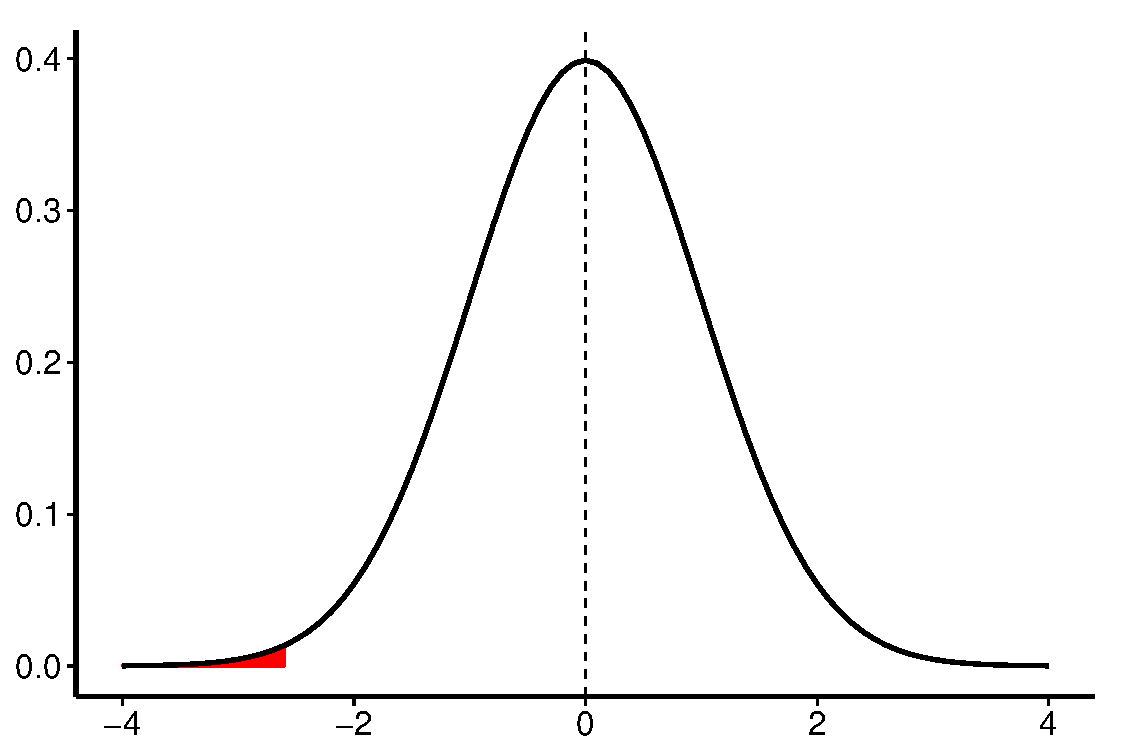
\includegraphics[width=\maxwidth,height=0.7\textheight]{figure/testez-1} 

\end{knitrout}

\end{frame} 
%===============================================================================%

%===============================================================================
\begin{frame}[fragile]{Teste Z -  Visualmente}

\begin{knitrout}
\definecolor{shadecolor}{rgb}{0.969, 0.969, 0.969}\color{fgcolor}
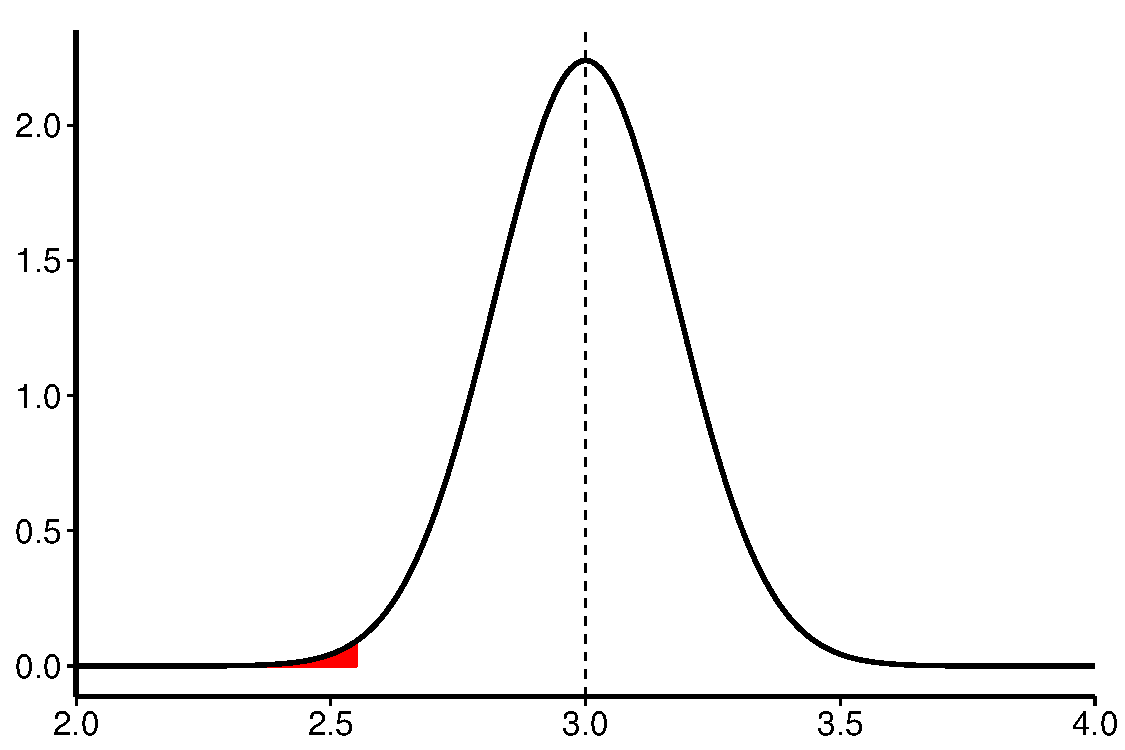
\includegraphics[width=\maxwidth,height=0.7\textheight]{figure/testez21-1} 

\end{knitrout}

\end{frame} 
%===============================================================================%

%===============================================================================
\begin{frame}{Exemplo: Teste Z para a média}

\begin{block}{Pergunta}

Estou interessado em saber se a concentração de clorofila varia entre dois reservatórios. 

O primeiro  tem um concentração de 2.5 mg.m$^{-3}$, e o segundo de 2.8 mg.m$^{-3}$ (diferença de 0.3 mg.m$^{-3}$). Qual a evidência de que as concentrações são diferentes? 

\end{block}

\end{frame} 
%===============================================================================%

%===============================================================================
\begin{frame}{Exemplo: Teste Z para a média}

\textbf{H$_0$:} Os reservatórios são iguais, então $\mu_1 = \mu_2$, ou $\mu_1 - \mu_2 = 0$
\vfill
\textbf{H$_1$:} Os reservatórios são diferentes, então $\mu_1 \neq \mu_2$, ou $\mu_1 - \mu_2 \neq 0$
\vfill
$P(\bar{X_1} -  \bar{X_1} >= 0.3 | \mu_1 - \mu_2 = 0)$?
\vfill

\textbf{Estatística:} $Z$

\vfill

\begin{equation*}
    Z = \frac{(\bar{X_1}-\bar{X_2}) - (\mu_1 - \mu_2)}{\sqrt{E.P._1^2 + E.P._2^2}} = \frac{(\bar{X_1}-\bar{X_2}) - (\mu_1 - \mu_2)}{\sqrt{\frac{\sigma_1^2}{n_1}} + \sqrt{\frac{\sigma_2^2}{n_2}}}
        
\end{equation*}

\end{frame} 
%===============================================================================%



%===============================================================================
\begin{frame}[fragile]{Exemplo: Teste Z para a média}

\begin{knitrout}\tiny
\definecolor{shadecolor}{rgb}{0.969, 0.969, 0.969}\color{fgcolor}\begin{kframe}
\begin{alltt}
\hlstd{n}\hlkwb{=}\hlnum{20}
\hlstd{x1} \hlkwb{<-}  \hlkwd{c}\hlstd{(}\hlnum{1.85}\hlstd{,} \hlnum{2.64}\hlstd{,} \hlnum{3.63}\hlstd{,} \hlnum{1.94}\hlstd{,} \hlnum{2.41}\hlstd{,} \hlnum{2.74}\hlstd{,} \hlnum{2.85}\hlstd{,} \hlnum{3.07}\hlstd{,} \hlnum{1.29}\hlstd{,}\hlnum{1.50}\hlstd{,} \hlnum{1.55}\hlstd{,} \hlnum{1.69}\hlstd{,}
         \hlnum{3.70}\hlstd{,} \hlnum{3.25}\hlstd{,} \hlnum{2.47}\hlstd{,} \hlnum{1.95}\hlstd{,} \hlnum{3.33}\hlstd{,} \hlnum{2.21}\hlstd{,} \hlnum{3.02}\hlstd{,} \hlnum{3.98}\hlstd{)}

\hlstd{x2} \hlkwb{<-} \hlkwd{c}\hlstd{(}\hlnum{2.79}\hlstd{,} \hlnum{2.61}\hlstd{,} \hlnum{3.72}\hlstd{,} \hlnum{1.58}\hlstd{,} \hlnum{2.02}\hlstd{,} \hlnum{2.38}\hlstd{,} \hlnum{2.70}\hlstd{,} \hlnum{3.18}\hlstd{,} \hlnum{3.96}\hlstd{,} \hlnum{1.53}\hlstd{,} \hlnum{1.51}\hlstd{,} \hlnum{2.08}\hlstd{,}
        \hlnum{3.34}\hlstd{,} \hlnum{3.76}\hlstd{,} \hlnum{2.61}\hlstd{,} \hlnum{3.98}\hlstd{,} \hlnum{3.50}\hlstd{,} \hlnum{2.34}\hlstd{,} \hlnum{2.95}\hlstd{,} \hlnum{3.91}\hlstd{)}

\hlstd{x_barra1} \hlkwb{=} \hlkwd{mean}\hlstd{(x1); x_barra2} \hlkwb{=} \hlkwd{mean}\hlstd{(x2)}

\hlstd{x_barra1; x_barra2}
\end{alltt}
\begin{verbatim}
## [1] 2.5535
## [1] 2.8225
\end{verbatim}
\begin{alltt}
\hlstd{s1} \hlkwb{=} \hlkwd{sd}\hlstd{(x1); s2}\hlkwb{=}\hlkwd{sd}\hlstd{(x2)}
\hlstd{s1;s2}
\end{alltt}
\begin{verbatim}
## [1] 0.7964016
## [1] 0.8284092
\end{verbatim}
\begin{alltt}
\hlstd{mu1} \hlkwb{=} \hlstd{mu2} \hlkwb{=} \hlnum{0}
\end{alltt}
\end{kframe}
\end{knitrout}
\end{frame} 
%===============================================================================%


%===============================================================================
\begin{frame}[fragile]{Exemplo: Teste Z para a média}

\begin{knitrout}\tiny
\definecolor{shadecolor}{rgb}{0.969, 0.969, 0.969}\color{fgcolor}\begin{kframe}
\begin{alltt}
\hlstd{z} \hlkwb{<-} \hlstd{((x_barra1}\hlopt{-}\hlstd{x_barra2)}\hlopt{-}\hlstd{(mu1}\hlopt{-}\hlstd{mu2))}\hlopt{/}\hlstd{(}\hlkwd{sqrt}\hlstd{(s1}\hlopt{^}\hlnum{2}\hlopt{/}\hlstd{n)}\hlopt{+}\hlkwd{sqrt}\hlstd{(s2}\hlopt{^}\hlnum{2}\hlopt{/}\hlstd{n))}
\hlstd{z}
\end{alltt}
\begin{verbatim}
## [1] -0.7403967
\end{verbatim}
\begin{alltt}
\hlkwd{pnorm}\hlstd{(z,}\hlnum{0}\hlstd{,}\hlnum{1}\hlstd{)}
\end{alltt}
\begin{verbatim}
## [1] 0.2295297
\end{verbatim}
\begin{alltt}
\hlcom{# Ou simplesmente}

\hlkwd{pnorm}\hlstd{(x_barra1}\hlopt{-}\hlstd{x_barra2,mu1}\hlopt{-}\hlstd{mu2,}\hlkwd{sqrt}\hlstd{(s1}\hlopt{^}\hlnum{2}\hlopt{/}\hlstd{n)}\hlopt{+}\hlkwd{sqrt}\hlstd{(s2}\hlopt{^}\hlnum{2}\hlopt{/}\hlstd{n))}
\end{alltt}
\begin{verbatim}
## [1] 0.2295297
\end{verbatim}
\end{kframe}
\end{knitrout}

\end{frame} 
%===============================================================================%

%===============================================================================
\begin{frame}[fragile]{Teste Z -  Visualmente}

\begin{knitrout}
\definecolor{shadecolor}{rgb}{0.969, 0.969, 0.969}\color{fgcolor}
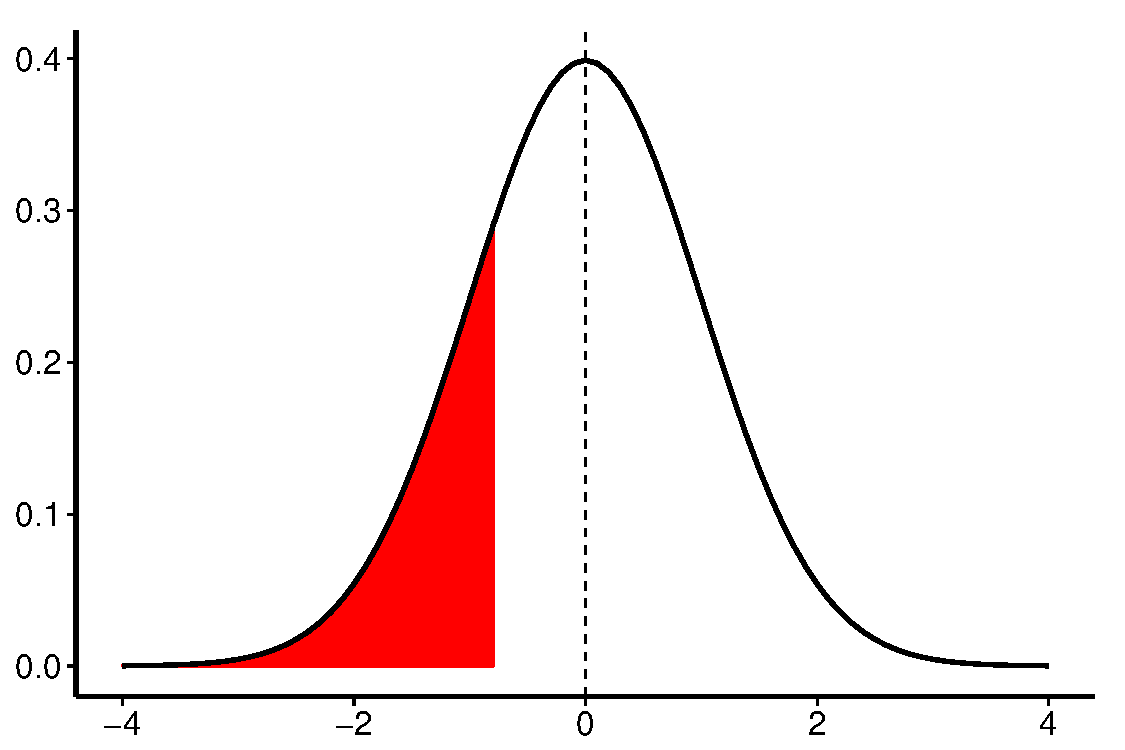
\includegraphics[width=\maxwidth,height=0.7\textheight]{figure/testez2-1} 

\end{knitrout}

\end{frame} 
%===============================================================================%



%===============================================================================
\begin{frame}{Exemplo: Teste Z para a média}

Mas isso é só metade da história...a princípio, não sabemos na realidade qual lago é maior e qual é menor, então temos que considerar tanto que $\mu_1 > \mu_2$ quanto $\mu_2 > \mu_1$.


\end{frame} 
%===============================================================================%


%===============================================================================
\begin{frame}[fragile]

\begin{knitrout}\tiny
\definecolor{shadecolor}{rgb}{0.969, 0.969, 0.969}\color{fgcolor}\begin{kframe}
\begin{alltt}
\hlstd{z_min} \hlkwb{<-} \hlstd{((x_barra1}\hlopt{-}\hlstd{x_barra2)}\hlopt{-}\hlstd{(mu1}\hlopt{-}\hlstd{mu2))}\hlopt{/}\hlstd{(}\hlkwd{sqrt}\hlstd{(s1}\hlopt{^}\hlnum{2}\hlopt{/}\hlstd{n)}\hlopt{+}\hlkwd{sqrt}\hlstd{(s2}\hlopt{^}\hlnum{2}\hlopt{/}\hlstd{n))}
\hlstd{z_max} \hlkwb{<-} \hlstd{((x_barra2}\hlopt{-}\hlstd{x_barra1)}\hlopt{-}\hlstd{(mu2}\hlopt{-}\hlstd{mu1))}\hlopt{/}\hlstd{(}\hlkwd{sqrt}\hlstd{(s2}\hlopt{^}\hlnum{2}\hlopt{/}\hlstd{n)}\hlopt{+}\hlkwd{sqrt}\hlstd{(s1}\hlopt{^}\hlnum{2}\hlopt{/}\hlstd{n))}

\hlkwd{pnorm}\hlstd{(z_min,}\hlnum{0}\hlstd{,}\hlnum{1}\hlstd{)}
\end{alltt}
\begin{verbatim}
## [1] 0.2295297
\end{verbatim}
\begin{alltt}
\hlkwd{pnorm}\hlstd{(z_max,}\hlnum{0}\hlstd{,}\hlnum{1}\hlstd{)}
\end{alltt}
\begin{verbatim}
## [1] 0.7704703
\end{verbatim}
\begin{alltt}
\hlstd{p_final} \hlkwb{<-} \hlkwd{pnorm}\hlstd{(z_min,}\hlnum{0}\hlstd{,}\hlnum{1}\hlstd{)} \hlopt{+} \hlstd{(}\hlnum{1} \hlopt{-} \hlkwd{pnorm}\hlstd{(z_max,}\hlnum{0}\hlstd{,}\hlnum{1}\hlstd{))}

\hlstd{p_final}
\end{alltt}
\begin{verbatim}
## [1] 0.4590593
\end{verbatim}
\end{kframe}
\end{knitrout}


\end{frame} 
%===============================================================================%

%===============================================================================
\begin{frame}[fragile]{Teste Z -  Visualmente}

\begin{knitrout}
\definecolor{shadecolor}{rgb}{0.969, 0.969, 0.969}\color{fgcolor}
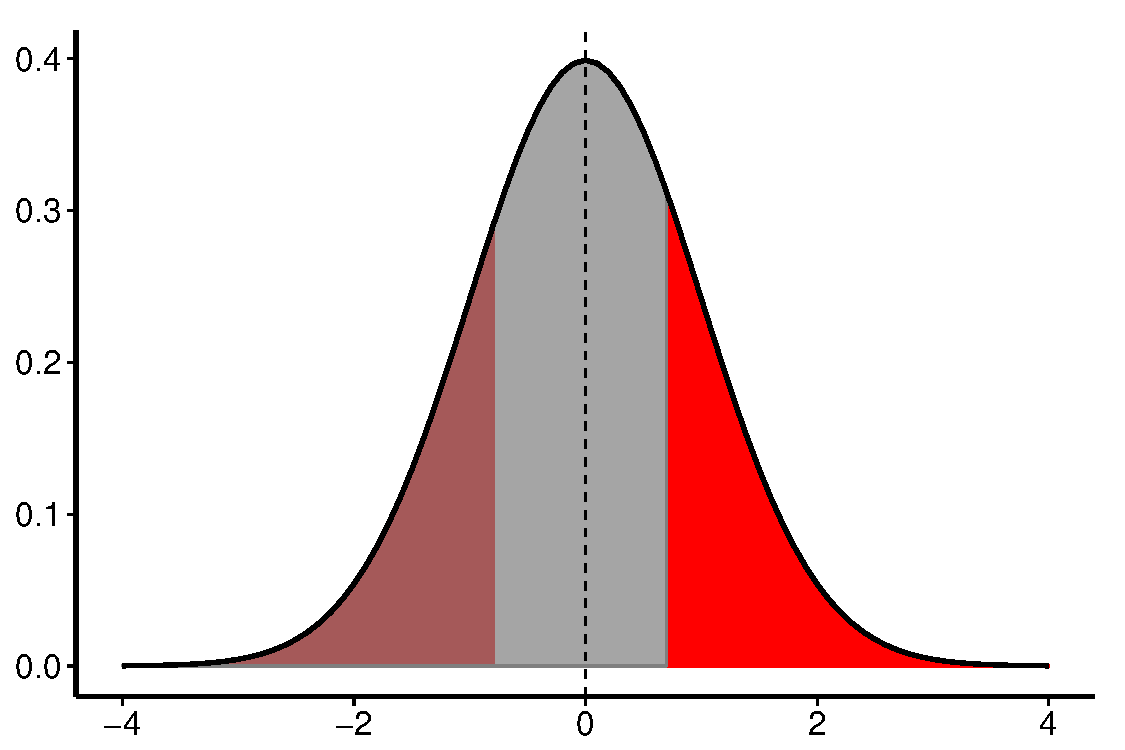
\includegraphics[width=\maxwidth,height=0.7\textheight]{figure/testez3-1} 

\end{knitrout}

\end{frame} 
%===============================================================================%

%===============================================================================
\begin{frame}{Problema do teste Z}

\begin{itemize}

\item Até agora, assumimos que o desvio padrão da amostra aproxima o desvio padrão da população. Mas quanto menor a amostra, menos isso é verdade.
\vfill
\begin{equation*}
    Z = \frac{\bar{X} - \mu}{\sigma / \sqrt{n}} \neq \frac{\bar{X} - \mu}{s / \sqrt{n}}
\end{equation*}
\vfill
\item O uso de $s$ em vez de $\sigma$ introduz um erro, ou o que chamamos de um \textbf{viés (bias)}
\vfill
\item Felizmente, existe uma maneira simples de corrigir esse viés:
\vfill
\item A distribuição \textbf{t de Student}

\end{itemize}

\end{frame} 
%===============================================================================%

%===============================================================================%
\begin{frame}{A distribuição $t$ de Student}

\begin{itemize}
  \item Student = William Gosset
  \vfill
  \item Pelo Teorema do Limite Central, $s$ aproxima $\sigma$ para "grandes" amostras ($n \geq 30$). Mas, se as amostras são pequenas, isso não vale.
  \vfill
  \item Para pequenas amostras, essa estatística se aproxima mais de uma distribuição $t$ de Student.
  \vfill
  \item O único parâmetro de $t$ é $\nu = (n-1)$, onde $n$ é o número de observações. Esse parametro é conhecido como "graus de liberdade".
  \vfill
  \item Quando ($n \geq 30$), $t$ se aproxima de uma distribuição normal.
  \vfill
\end{itemize}

\end{frame}
%===============================================================================%


%===============================================================================%
\begin{frame}[fragile]

\begin{knitrout}
\definecolor{shadecolor}{rgb}{0.969, 0.969, 0.969}\color{fgcolor}
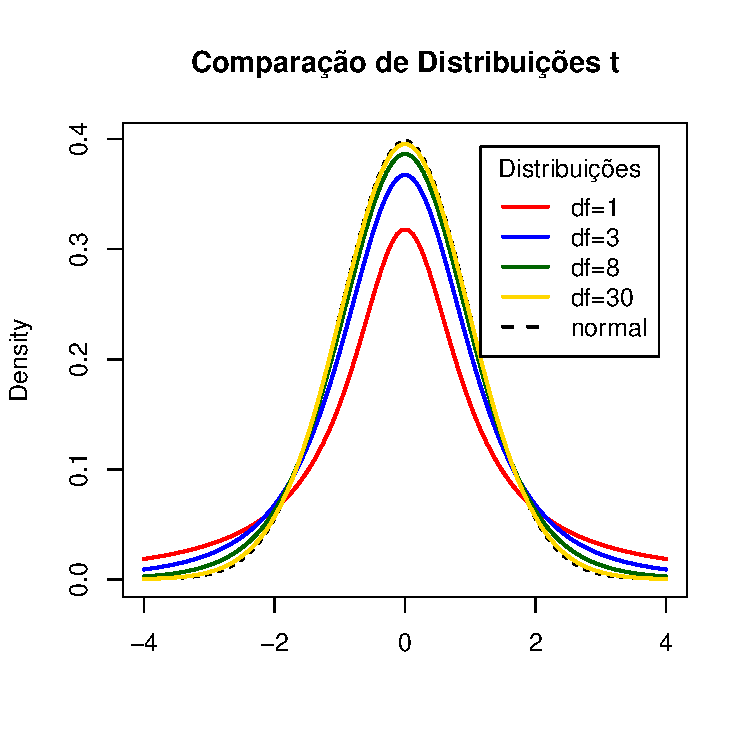
\includegraphics[width=0.8\linewidth]{figure/unnamed-chunk-11-1} 

\end{knitrout}



\end{frame}
%===============================================================================%


%===============================================================================
\begin{frame}[fragile]{Corrigindo nossos exemplos anteriores}

\begin{knitrout}\tiny
\definecolor{shadecolor}{rgb}{0.969, 0.969, 0.969}\color{fgcolor}\begin{kframe}
\begin{alltt}
\hlstd{t} \hlkwb{<-} \hlstd{(x_barra}\hlopt{-}\hlstd{mu)}\hlopt{/}\hlstd{(s}\hlopt{/}\hlkwd{sqrt}\hlstd{(n))}

\hlkwd{pnorm}\hlstd{(t,}\hlnum{0}\hlstd{,}\hlnum{1}\hlstd{);}\hlkwd{pt}\hlstd{(t,n}\hlopt{-}\hlnum{1}\hlstd{)} \hlcom{# neste caso, chamamos a estatística de t, e não z}
\end{alltt}
\begin{verbatim}
## [1] 0.006083066
## [1] 0.01070439
\end{verbatim}
\begin{alltt}
\hlcom{# ou, usando o comando interno do R}
\hlkwd{t.test}\hlstd{(x,}\hlkwc{mu}\hlstd{=}\hlnum{3}\hlstd{,}\hlkwc{alternative}\hlstd{=}\hlstr{'less'}\hlstd{)}
\end{alltt}
\begin{verbatim}
## 
## 	One Sample t-test
## 
## data:  x
## t = -2.5073, df = 19, p-value = 0.0107
## alternative hypothesis: true mean is less than 3
## 95 percent confidence interval:
##      -Inf 2.861425
## sample estimates:
## mean of x 
##    2.5535
\end{verbatim}
\end{kframe}
\end{knitrout}
\end{frame} 
%===============================================================================%


%===============================================================================
\begin{frame}[fragile]{Corrigindo nossos exemplos anteriores}

\begin{knitrout}\tiny
\definecolor{shadecolor}{rgb}{0.969, 0.969, 0.969}\color{fgcolor}\begin{kframe}
\begin{alltt}
\hlstd{t} \hlkwb{<-} \hlstd{((x_barra1}\hlopt{-}\hlstd{x_barra2)}\hlopt{-}\hlstd{(mu1}\hlopt{-}\hlstd{mu2))}\hlopt{/}\hlkwd{sqrt}\hlstd{((s1}\hlopt{^}\hlnum{2}\hlopt{/}\hlstd{n1)}\hlopt{+}\hlstd{(s2}\hlopt{^}\hlnum{2}\hlopt{/}\hlstd{n2))}

\hlkwd{pnorm}\hlstd{(t,}\hlnum{0}\hlstd{,}\hlnum{1}\hlstd{);} \hlkwd{pt}\hlstd{(t,n}\hlopt{-}\hlnum{1}\hlstd{)}
\end{alltt}
\begin{verbatim}
## [1] 0.1475784
## [1] 0.1541463
\end{verbatim}
\begin{alltt}
\hlkwd{t.test}\hlstd{(x1,x2,} \hlkwc{alternative}\hlstd{=}\hlstr{"less"}\hlstd{)}
\end{alltt}
\begin{verbatim}
## 
## 	Welch Two Sample t-test
## 
## data:  x1 and x2
## t = -1.0469, df = 37.941, p-value = 0.1509
## alternative hypothesis: true difference in means is less than 0
## 95 percent confidence interval:
##       -Inf 0.1642312
## sample estimates:
## mean of x mean of y 
##    2.5535    2.8225
\end{verbatim}
\end{kframe}
\end{knitrout}

\end{frame} 
%===============================================================================%

%===============================================================================%
\begin{frame}{Variações do teste $t$}

Teste $t$ para amostras independentes e variância conhecida: 
\vfill

\begin{scriptsize}
\begin{tabular}{ c c c }

$\bar{D} = \bar{X} - \bar{Y}$ & $Var(\bar{D}) = \sigma^{2}_{1}/n_1 + \sigma^{2}_{2}/n_2$ & $\frac{\bar{D}-\mu_D}{\sqrt{\sigma^{2}_{1}/n_1 + \sigma^{2}_{2}/n_2}} \sim N(0,1)$   \\

\end{tabular}
\end{scriptsize}

\vfill

Teste $t$ para amostras independentes e variância desconhecidas e iguais: 
\vfill

\begin{scriptsize}
\begin{tabular}{ c c c }

$\bar{D} = \bar{X} - \bar{Y}$ & $ S^{2}_{c} = \frac{(n_1-1)S^{2}_{X}+(n_2-1)S^{2}_{Y}}{(n_1-1)+(n_2-1)}$ & $\frac{\bar{D}-\mu_D}{\sqrt{S^{2}_{c}(1/n_1 + 1/n_2)}} \sim t_{(n_1+n_2-2)}$   \\

\end{tabular}
\end{scriptsize}

\end{frame}
%===============================================================================%

%===============================================================================%
\begin{frame}{Variações do teste $t$}

Teste $t$ para amostras independentes e variância desconhecidas e diferentes: 
\vfill

\begin{scriptsize}
\begin{tabular}{ c c c }

$\bar{D} = \bar{X} - \bar{Y}$ & $ \hat{S}^{2}= S^{2}_{X}/n_1 + S^{2}_{Y}/n_2$ & $\frac{\bar{D}-\mu_D}{\sqrt{S^{2}_{X}/n_1 + S^{2}_{Y}/n_2)}} \sim t_{(\nu)}$   \\

\end{tabular}
\end{scriptsize}

\vfill

Teste $t$ para amostras pareadas
\vfill

\begin{scriptsize}
\begin{tabular}{ c c c }

$\bar{D} = \frac{\sum{D_i}}{N}$ & $ S^{2}_{D}= \frac{1}{n-1}\sum{D_i - \bar{D}}$ & $\frac{\bar{D}-\mu_D}{\sqrt{S^{2}_{D}/n}} \sim t_{(n-1)}$   \\

\end{tabular}
\end{scriptsize}

\end{frame}
%===============================================================================%

\section{Erros Tipo I ($\alpha$) e Tipo II ($\beta$)}

%===============================================================================%
\begin{frame}{Erros Tipo I ($\alpha$) e Tipo II ($\beta$)}

\alert{LEMBRETE IMPORTANTE:} o teste é sempre baseado na distribuição amostral da estatística de interesse, e não na distribuição dos dados originais!


\end{frame}
%===============================================================================%
% 




%===============================================================================%
\begin{frame}{Erros Tipo I ($\alpha$)}

Imaginemos um teste $z$ para comparação das médias de duas amostras:
\vfill
$X_1 \sim N(\mu=10,\sigma=5)$ e $X_2 \sim N(\mu=12,\sigma=5)$. 
\vfill
Cada população foi amostrada com $n = 30$.
\vfill  
\begin{knitrout}\small
\definecolor{shadecolor}{rgb}{0.969, 0.969, 0.969}\color{fgcolor}\begin{kframe}
\begin{alltt}
\hlkwd{set.seed}\hlstd{(}\hlnum{1979}\hlstd{)}

\hlstd{x1} \hlkwb{<-} \hlkwd{rnorm}\hlstd{(}\hlnum{30}\hlstd{,} \hlnum{10}\hlstd{,} \hlnum{5}\hlstd{)}

\hlstd{x2} \hlkwb{<-} \hlkwd{rnorm}\hlstd{(}\hlnum{30}\hlstd{,} \hlnum{12}\hlstd{,} \hlnum{5}\hlstd{)}
\end{alltt}
\end{kframe}
\end{knitrout}


\end{frame}
%===============================================================================%



%===============================================================================%
\begin{frame}[fragile]{Erros Tipo I ($\alpha$)}


Como sabemos, $\bar{X}$ e $s$ aproximam (estimam) $\mu$ e $\sigma$. Quanto maior o $n$, melhor a estimação.

\vfill

\begin{columns}[c]
\column{.5\textwidth}
\begin{knitrout}\small
\definecolor{shadecolor}{rgb}{0.969, 0.969, 0.969}\color{fgcolor}\begin{kframe}
\begin{alltt}
\hlkwd{mean}\hlstd{(x1)}
\end{alltt}
\begin{verbatim}
## [1] 9.413282
\end{verbatim}
\begin{alltt}
\hlkwd{mean}\hlstd{(x2)}
\end{alltt}
\begin{verbatim}
## [1] 12.40707
\end{verbatim}
\end{kframe}
\end{knitrout}

\column{.5\textwidth}
\begin{knitrout}\small
\definecolor{shadecolor}{rgb}{0.969, 0.969, 0.969}\color{fgcolor}\begin{kframe}
\begin{alltt}
\hlkwd{sd}\hlstd{(x1)}
\end{alltt}
\begin{verbatim}
## [1] 5.012927
\end{verbatim}
\begin{alltt}
\hlkwd{sd}\hlstd{(x2)}
\end{alltt}
\begin{verbatim}
## [1] 3.540709
\end{verbatim}
\end{kframe}
\end{knitrout}

\end{columns}

\end{frame}
%===============================================================================%


%===============================================================================%
\begin{frame}{Erros Tipo I ($\alpha$)}

Poderíamos formular duas hipóteses
\vfill

$H_1$: $\mu_1 - \mu_2 = 0$

$H_2$: $\mu_1 - \mu_2 = 2$

\vfill

Neste caso, a nossa $H_2$ corresponde exatamente à realidade, mas só para fins didáticos.

\end{frame}
%===============================================================================%

%===============================================================================%
\begin{frame}[fragile]{Erros Tipo I ($\alpha$)}

\small{Podemos até visualizar como $X_1$ e $X_2$ estão distribuídos:}

\begin{knitrout}\tiny
\definecolor{shadecolor}{rgb}{0.969, 0.969, 0.969}\color{fgcolor}\begin{kframe}
\begin{alltt}
\hlkwd{curve}\hlstd{(}\hlkwd{dnorm}\hlstd{(x,} \hlkwc{mean} \hlstd{=} \hlnum{10}\hlstd{,} \hlkwc{sd} \hlstd{=} \hlnum{5}\hlstd{),} \hlopt{-}\hlnum{10}\hlstd{,} \hlnum{35}\hlstd{, ,} \hlkwc{col} \hlstd{=} \hlstr{"blue"}\hlstd{,} \hlkwc{cex} \hlstd{=} \hlnum{2}\hlstd{)}
\hlkwd{curve}\hlstd{(}\hlkwd{dnorm}\hlstd{(x,} \hlkwc{mean} \hlstd{=} \hlnum{15}\hlstd{,} \hlkwc{sd} \hlstd{=} \hlnum{5}\hlstd{),} \hlopt{-}\hlnum{10}\hlstd{,} \hlnum{35}\hlstd{, ,} \hlkwc{col} \hlstd{=} \hlstr{"red"}\hlstd{,} \hlkwc{add} \hlstd{= T)}
\end{alltt}
\end{kframe}
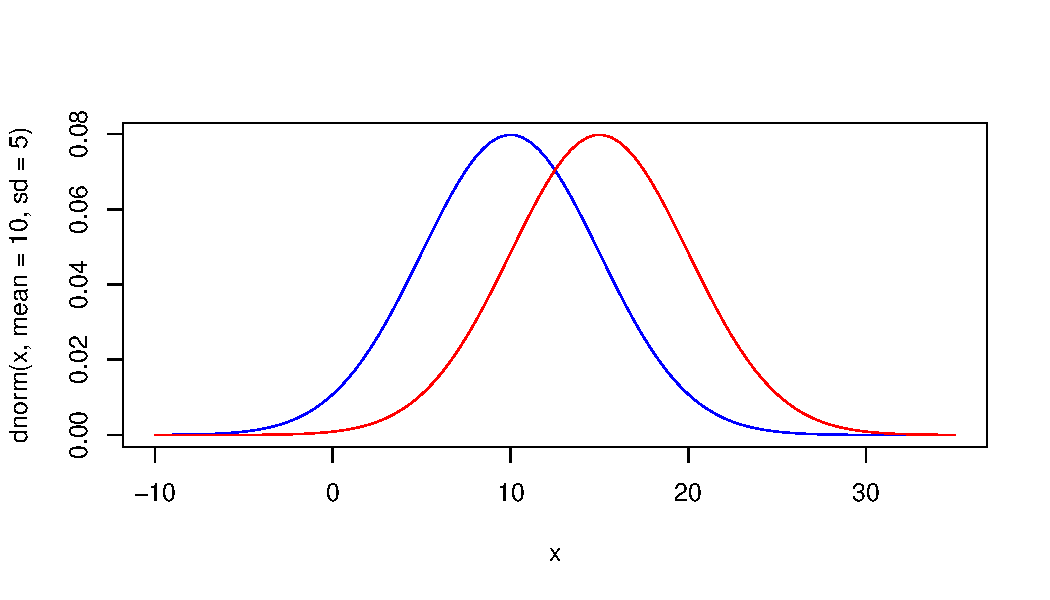
\includegraphics[width=\maxwidth]{figure/erro_alfa_4-1} 

\end{knitrout}


\end{frame}
%===============================================================================%


%===============================================================================%
\begin{frame}[fragile]{Erros Tipo I ($\alpha$)}

\small{Mas o nosso teste se baseia na distribuição amostral da estatística ($\bar{X}_D - \mu_D$), e não das variáveis ($\bar{X_1}$ e $\bar{X_2}).}

\center{Lembrando: $\sigma_{\mu} = \dfrac{\sigma}{\sqrt{N}}$}

\vfill
\begin{knitrout}\small
\definecolor{shadecolor}{rgb}{0.969, 0.969, 0.969}\color{fgcolor}\begin{kframe}
\begin{alltt}
\hlstd{h1.mu} \hlkwb{<-} \hlnum{0}

\hlstd{h2.mu} \hlkwb{<-} \hlnum{2}

\hlstd{h1.err} \hlkwb{<-} \hlstd{h2.err} \hlkwb{<-} \hlnum{5}\hlopt{/}\hlkwd{sqrt}\hlstd{(}\hlnum{30}\hlstd{)}
\end{alltt}
\end{kframe}
\end{knitrout}


\end{frame}
%===============================================================================%


%===============================================================================%
\begin{frame}[fragile]{Erros Tipo I ($\alpha$)}

\begin{knitrout}\tiny
\definecolor{shadecolor}{rgb}{0.969, 0.969, 0.969}\color{fgcolor}\begin{kframe}
\begin{alltt}
\hlkwd{curve}\hlstd{(}\hlkwd{dnorm}\hlstd{(x,} \hlkwc{mean} \hlstd{= h2.mu,} \hlkwc{sd} \hlstd{= h1.err),} \hlopt{-}\hlnum{10}\hlstd{,} \hlnum{10}\hlstd{, ,} \hlkwc{col} \hlstd{=} \hlstr{"red"}\hlstd{)}
\end{alltt}
\end{kframe}
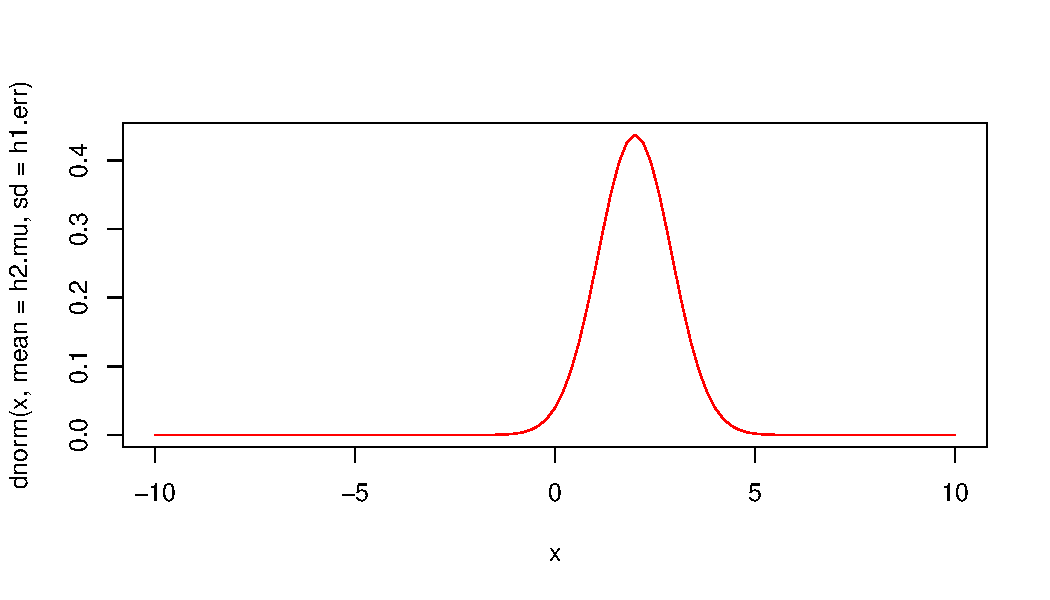
\includegraphics[width=\maxwidth]{figure/erro_alfa_6-1} 
\begin{kframe}\begin{alltt}
\hlkwd{curve}\hlstd{(}\hlkwd{dnorm}\hlstd{(x,} \hlkwc{mean} \hlstd{= h1.mu,} \hlkwc{sd} \hlstd{= h0.err),} \hlopt{-}\hlnum{10}\hlstd{,} \hlnum{10}\hlstd{, ,} \hlkwc{col} \hlstd{=} \hlstr{"blue"}\hlstd{,} \hlkwc{add} \hlstd{= T)}
\end{alltt}


{\ttfamily\noindent\bfseries\color{errorcolor}{\#\# Error in dnorm(x, mean = h1.mu, sd = h0.err): object 'h0.err' not found}}\end{kframe}
\end{knitrout}

\end{frame}
%===============================================================================%


%===============================================================================%
\begin{frame}{Erros Tipo I ($\alpha$)}

O teste de hipótese clássico ("ritual nulo"), como vimos, só se baseia em refutar uma das hipóteses, independente de outras hipóteses.

\begin{enumerate}
  \item Definimos a estatística de interesse: $(\bar{X}_D - \mu_D)/E.P.$ ($H_1: \mu_D = 0$)
  \item Estimamos a estatística com base na amostra
  \item Assumimos uma distribuição para essa estatística ($z$)
  \item Estabelecemos nosso nível de significância ($\alpha = 5\%$)
  \item Calculamos a probabilidade de observarmos uma estatística $z$ maior ou igual ao valor crítico ($P(z \geq z_{0.05}$)
  \item Com base nesse probabilidade, rejeitamos ou não a hipótese
\end{enumerate}

\end{frame}
%===============================================================================%


%===============================================================================%
\begin{frame}[fragile]{Erros Tipo I ($\alpha$)}

Para o nosso caso:

Valor Z calculado:

\begin{knitrout}\tiny
\definecolor{shadecolor}{rgb}{0.969, 0.969, 0.969}\color{fgcolor}\begin{kframe}
\begin{alltt}
\hlstd{z}\hlkwb{<-} \hlstd{((}\hlkwd{mean}\hlstd{(x2)}\hlopt{-}\hlkwd{mean}\hlstd{(x1))} \hlopt{-} \hlnum{0}\hlstd{)}\hlopt{/} \hlstd{(}\hlnum{5}\hlopt{/}\hlkwd{sqrt}\hlstd{(}\hlnum{30}\hlstd{)); z}
\end{alltt}
\begin{verbatim}
## [1] 3.279533
\end{verbatim}
\end{kframe}
\end{knitrout}

Valor Z associado à probabilidade de 0.05: 

\begin{knitrout}\tiny
\definecolor{shadecolor}{rgb}{0.969, 0.969, 0.969}\color{fgcolor}\begin{kframe}
\begin{alltt}
\hlstd{z_005} \hlkwb{<-} \hlkwd{qnorm}\hlstd{(}\hlnum{0.05}\hlstd{,}\hlnum{0}\hlstd{,}\hlnum{1}\hlstd{,}\hlkwc{lower.tail}\hlstd{=F); z_005}
\end{alltt}
\begin{verbatim}
## [1] 1.644854
\end{verbatim}
\end{kframe}
\end{knitrout}
\end{frame}
%===============================================================================%


%===============================================================================%
\begin{frame}[fragile]{Erros Tipo I ($\alpha$)}

\begin{knitrout}\tiny
\definecolor{shadecolor}{rgb}{0.969, 0.969, 0.969}\color{fgcolor}\begin{kframe}
\begin{alltt}
\hlkwd{curve}\hlstd{(}\hlkwd{dnorm}\hlstd{(x,} \hlkwc{mean} \hlstd{= h2.mu,} \hlkwc{sd} \hlstd{= h2.err),} \hlopt{-}\hlnum{10}\hlstd{,} \hlnum{10}\hlstd{, ,} \hlkwc{col} \hlstd{=} \hlstr{"red"}\hlstd{)}
\hlkwd{curve}\hlstd{(}\hlkwd{dnorm}\hlstd{(x,} \hlkwc{mean} \hlstd{= h1.mu,} \hlkwc{sd} \hlstd{= h1.err),} \hlopt{-}\hlnum{10}\hlstd{,} \hlnum{10}\hlstd{, ,} \hlkwc{col} \hlstd{=} \hlstr{"blue"}\hlstd{,} \hlkwc{add} \hlstd{= T)}
\hlkwd{abline}\hlstd{(}\hlkwc{v} \hlstd{= z_005,} \hlkwc{col} \hlstd{=} \hlstr{"blue"}\hlstd{)}
\hlkwd{abline}\hlstd{(}\hlkwc{v} \hlstd{= z,} \hlkwc{lty} \hlstd{=} \hlnum{1}\hlstd{)}
\end{alltt}
\end{kframe}
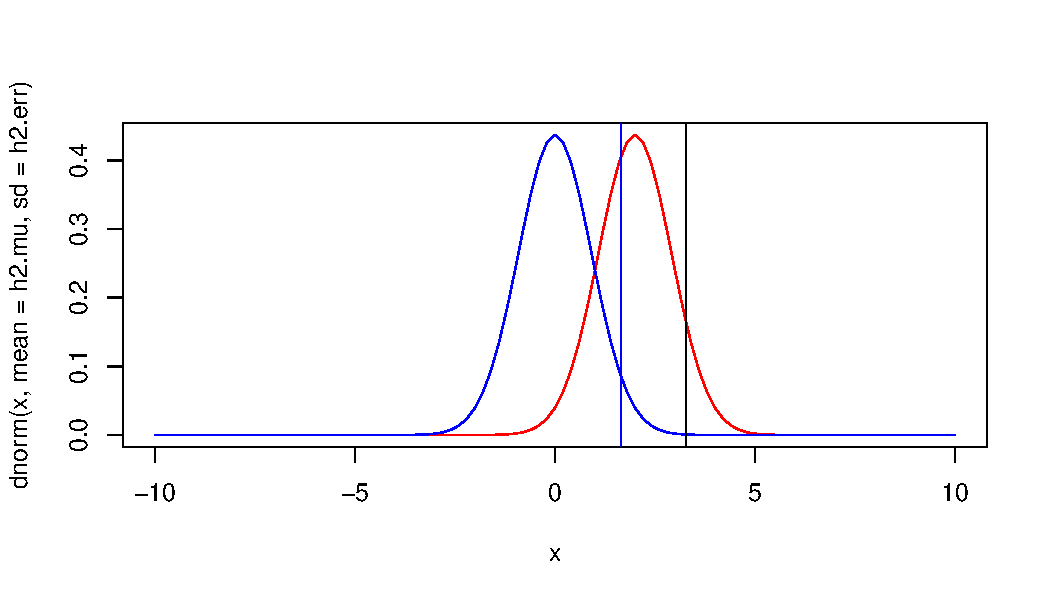
\includegraphics[width=\maxwidth]{figure/erro_alfa_7-1} 

\end{knitrout}

\end{frame}
%===============================================================================%


%===============================================================================%
\begin{frame}[fragile]{Erros Tipo I ($\alpha$)}

Apesar de não ser comum, nada impede que testemos diferentes hipóteses "competitivas", por exemplo, $H_2: \mu_D = 2$
\vfill
\begin{knitrout}\tiny
\definecolor{shadecolor}{rgb}{0.969, 0.969, 0.969}\color{fgcolor}\begin{kframe}
\begin{alltt}
\hlstd{z}\hlkwb{<-} \hlstd{((}\hlkwd{mean}\hlstd{(x2)}\hlopt{-}\hlkwd{mean}\hlstd{(x1))} \hlopt{-} \hlnum{2}\hlstd{)}\hlopt{/} \hlstd{(}\hlnum{5}\hlopt{/}\hlkwd{sqrt}\hlstd{(}\hlnum{30}\hlstd{)); z}
\end{alltt}
\begin{verbatim}
## [1] 1.088642
\end{verbatim}
\begin{alltt}
\hlstd{z_005} \hlkwb{<-} \hlkwd{qnorm}\hlstd{(}\hlnum{0.05}\hlstd{,}\hlnum{2}\hlstd{,}\hlnum{1}\hlstd{,}\hlkwc{lower.tail}\hlstd{=F); z_005}
\end{alltt}
\begin{verbatim}
## [1] 3.644854
\end{verbatim}
\end{kframe}
\end{knitrout}

\end{frame}
%===============================================================================%


%===============================================================================%
\begin{frame}[fragile]{Erros Tipo I ($\alpha$)}

\begin{knitrout}\tiny
\definecolor{shadecolor}{rgb}{0.969, 0.969, 0.969}\color{fgcolor}\begin{kframe}
\begin{alltt}
\hlkwd{curve}\hlstd{(}\hlkwd{dnorm}\hlstd{(x,} \hlkwc{mean} \hlstd{= h2.mu,} \hlkwc{sd} \hlstd{= h2.err),} \hlopt{-}\hlnum{10}\hlstd{,} \hlnum{10}\hlstd{, ,} \hlkwc{col} \hlstd{=} \hlstr{"red"}\hlstd{)}
\hlkwd{curve}\hlstd{(}\hlkwd{dnorm}\hlstd{(x,} \hlkwc{mean} \hlstd{= h1.mu,} \hlkwc{sd} \hlstd{= h1.err),} \hlopt{-}\hlnum{10}\hlstd{,} \hlnum{10}\hlstd{, ,} \hlkwc{col} \hlstd{=} \hlstr{"blue"}\hlstd{,} \hlkwc{add} \hlstd{= T)}
\hlkwd{abline}\hlstd{(}\hlkwc{v} \hlstd{= z_005,} \hlkwc{col} \hlstd{=} \hlstr{"red"}\hlstd{)}
\hlkwd{abline}\hlstd{(}\hlkwc{v} \hlstd{= z,} \hlkwc{lty} \hlstd{=} \hlnum{1}\hlstd{)}
\end{alltt}
\end{kframe}
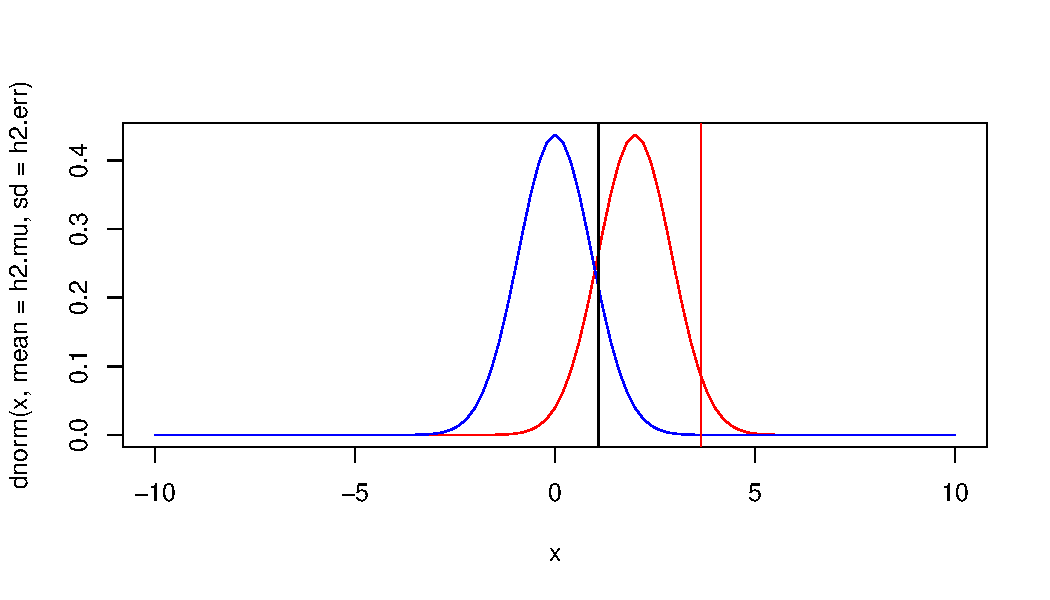
\includegraphics[width=\maxwidth]{figure/erro2-1} 

\end{knitrout}

\end{frame}
%===============================================================================%


%===============================================================================%
\begin{frame}[fragile]{Erros Tipo I ($\alpha$)}

\small{O erro Tipo I, ou erro $\alpha$, é a probabilidade de rejeitarmos $H_1$ em favor de $H_2$, quando $H_1$ é verdadeira. Ao estabelecermos um nível de significancia, decidimos qual porcentagem de erro Tipo I é aceitável:}

\begin{knitrout}\tiny
\definecolor{shadecolor}{rgb}{0.969, 0.969, 0.969}\color{fgcolor}
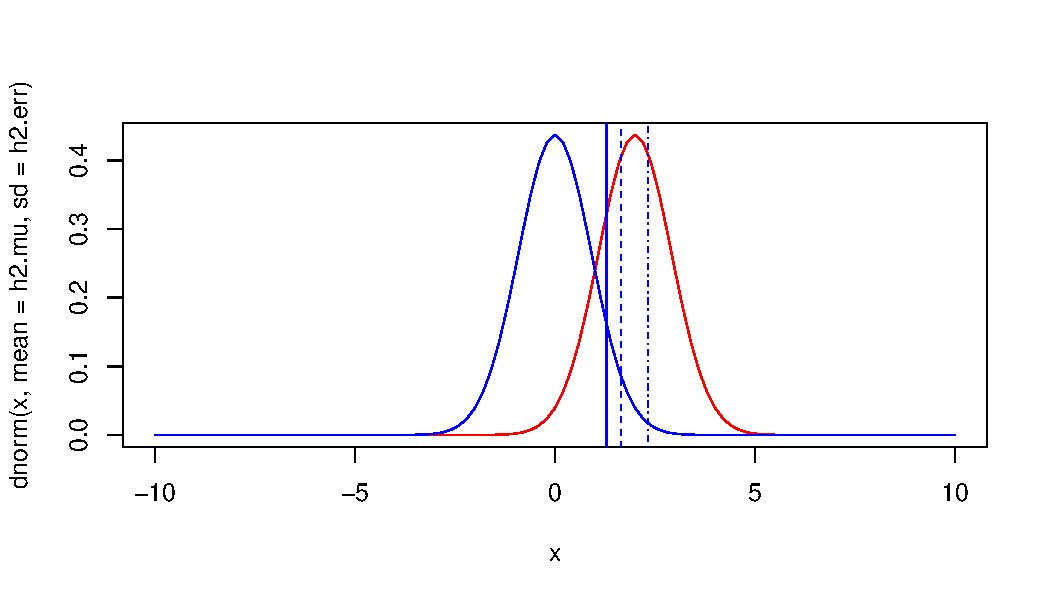
\includegraphics[width=\maxwidth]{figure/erro3-1} 

\end{knitrout}


\end{frame}
%===============================================================================%



%===============================================================================%
\begin{frame}{Erros Tipo II ($\beta$)}

\small{Contudo, podemos observar que existe um outro tipo possível de erro: rejeitar $H_2$ em favor de $H_1$, quando na verdade $H_2$ é verdadeira. Esse é o chamado erro Tipo II ($\beta$), também conhecido como \textbf{poder (\emph{power})} do teste.}

\begin{knitrout}\tiny
\definecolor{shadecolor}{rgb}{0.969, 0.969, 0.969}\color{fgcolor}
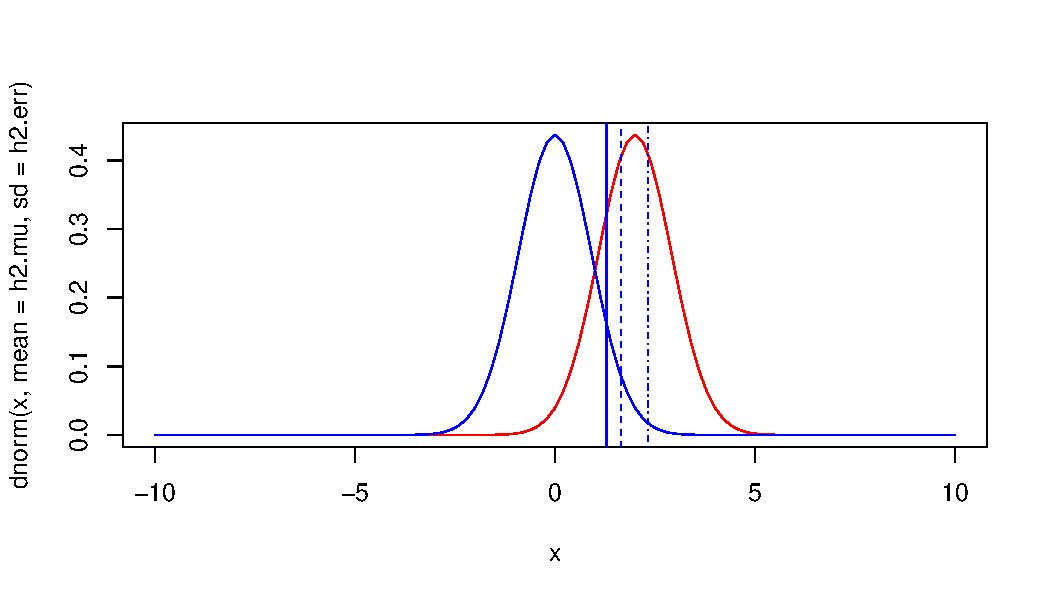
\includegraphics[width=\maxwidth]{figure/erro5-1} 

\end{knitrout}

\end{frame}
%===============================================================================%

%===============================================================================%
\begin{frame}{Erros Tipo II ($\beta$)}

E agora? Se aumentamos o nível de significância, perdemos poder. 

Seria esse o momento de abandonar de vez a ciência, e vender arte na praia? \pause

Como poderíamos resolver esse problema? \pause

\begin{enumerate}

  \item Avaliando efeitos maiores
  
  \item Reduzindo a nossa variância

\end{enumerate}

\end{frame}
%=======


%===============================================================================%
\begin{frame}[fragile]{Erros Tipo II ($\beta$)}

Avaliando efeitos maiores: $\mu_D = 6$

\begin{knitrout}\tiny
\definecolor{shadecolor}{rgb}{0.969, 0.969, 0.969}\color{fgcolor}
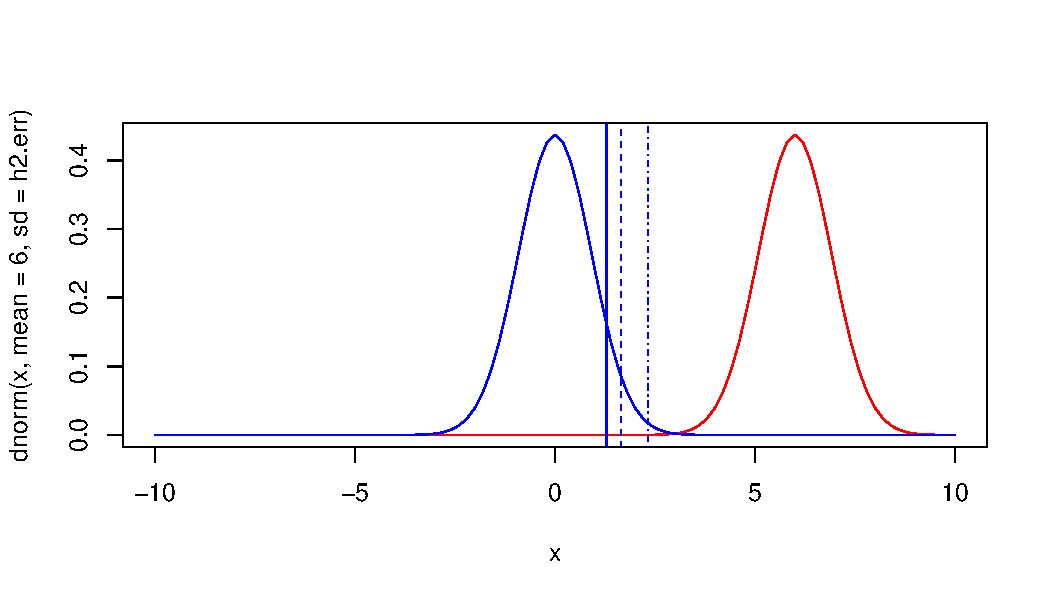
\includegraphics[width=\maxwidth]{figure/erro4-1} 

\end{knitrout}

\end{frame}
%===============================================================================%

%===============================================================================%
\begin{frame}[fragile]{Erros Tipo II ($\beta$)}

Aumentando a amostragem: n = 100, $\sigma_{\mu} = \dfrac{\sigma}{\sqrt{N}}$

\vfill


\begin{knitrout}\tiny
\definecolor{shadecolor}{rgb}{0.969, 0.969, 0.969}\color{fgcolor}
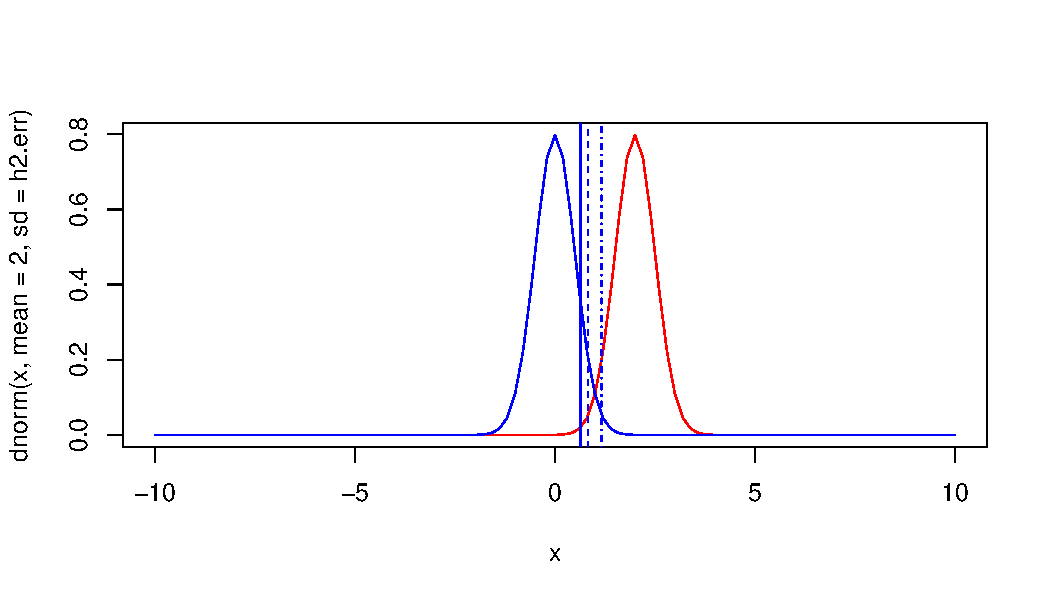
\includegraphics[width=\maxwidth]{figure/erro8-1} 

\end{knitrout}

\end{frame}
%===============================================================================%



%===============================================================================%
\begin{frame}{Estimando o tamanho amostral}

Esta relação nos permite estimar o esforço amostral necessário para garantir que tenhamos poder estatístico suficiente para detectar um efeito de tamanho $d$, com base na definição dos erros $\alpha$ e $\beta$ e em uma estimativa de $\sigma$.
  
  \vfill
  
  
  A maneira ideal de determinar os parâmetros necessários é a realização de um estudo piloto. Mas podemos também recorrer à literatura e/ou ao bom senso.

\end{frame}
%===============================================================================%




% 
% %===============================================================================
% \begin{frame}{Teorema do Limite Central}
% 
% \begin{itemize}
%   \item Seja $X$ uma v.a. independente e identicamente distribuída (i.i.d.), que possui esperança $E[X]=\mu$ e variância $Var[X]=\sigma$ \pause
%   \item Podemos tomar várias amostras de $X$ ($X_i$), com tamanho $n$, e calcular $E[X]_n$ para cada uma.\pause
%   \item Se nós normalizarmos as médias com relação à média original,
%     \begin{equation*}
%     Z_n = \frac{E[x]_n - \mu}{\sigma / \sqrt{n}}
%   \end{equation*}
%   \pause
%   
%   \item Então Z \sim N (0,1)$ ! 
% \end{itemize}
% 
%     
% \end{frame} 
% %===============================================================================%
% 
% %===============================================================================
% \begin{frame}[fragile]
% 
% \begin{columns}[c]
% 
% \column{0.5\linewidth}
% 
% <<size='tiny',eval=F>>=
% set.seed(1979)
% dados <- runif(500,1,6)
% hist(dados,main=NA)
% 
% means <- vector(100,mode='numeric')
% for (i in c(1:100)){
%   samp <- runif(5,1,6)
%   means[i] <- mean(samp)
% }
% 
% hist(means,breaks=10,main=NA)
% @
% 
% \column{0.5\linewidth}
% 
% <<fig.width=4,fig.height=3.5,out.width='0.9\\linewidth', echo=FALSE>>=
% set.seed(1979)
% dados <- runif(500,1,6)
% hist(dados,main=NA)
% 
% means <- vector(100,mode='numeric')
% for (i in c(1:100)){
%   samp <- runif(5,1,6)
%   means[i] <- mean(samp)
% }
% 
% hist(means,breaks=10,main=NA)
% @
% 
% \end{columns}
% 
% \end{frame} 
% %===============================================================================%
% 
% %===============================================================================
% \begin{frame}{Teorema do Limite Central}
% 
% \begin{itemize}
%   \item O teorema do limite central é uma das bases da inferência estatística paramétrica
%   \item Não importa a distribuição dos dados originais, a distribuição da média será aproximadamente normal se $n$ for grande 
%   \item Geralmente, estamos fazendo inferências sobre a média
%   \begin{itemize}
%     \item $\mu_1 > \mu_2$?
%     \item $\mu_1 - \mu_2 > 10$?
%     \item etc.
%     \end{itemize}
% \end{itemize}
% 
%     
% \end{frame} 
% %===============================================================================%
% 
% 
% 


%===============================================================================%
%===============================================================================%
%===============================================================================%
\end{document}
%===============================================================================%
%===============================================================================%
%===============================================================================%
